% Emmanuel Ren PhD thesis -- (C) 2023
%!TeX root = 2-thermo
\documentclass[main]{subfiles}

\begin{document}

\chapter{Thermodynamic exploration of xenon/krypton separation}
\vspace*{-1\baselineskip}

\section{Calculation of thermodynamic descriptors}

\subsection{Grand Canonical Monte Carlo}

%intro 
As explained before, we can think of adsorption as a gas--solid or liquid--solide interfacial phenomenon, the adsorbate phase fills the accessible pore volumes depending on the physical conditions the material is put under. No simple model can predict how the adsorbates would interact with the pore surface, how many of them can fit in, what configuration is the most stable, etc. To answer these questions, we can evaluate all possible adsorption configurations that would undeniably have different numbers of adsorbate, and only keep the most thermodynamically plausible ones. To do so, these configurations will have to follow a given probability distribution, the grand canonical ensemble probability for instance, because it allows the variation of the number of molecules (adsorbate molecules) and the total energy. With the help of a Monte Carlo simulation, we can vary the energy and the loading inside the pores so that the distribution of configurations $c$ follows this probability law: 
\begin{equation}
  P_c = \dfrac{1}{\Xi}e^{-\beta\left(E_c-\mu N_c\right)} 
  \label{eqn:gc}
\end{equation}
where $E_c$ and $N_c$ are respectively the energy and the number of adsorbate particles in the configuration $c$. Normally the energy and the number of molecules of all particles should be considered, but for now, since the whole system is considered rigid we will only focus on the adsorbate molecules. The chemical potential $\mu$ and the temperature $T$ inside of $\beta$ correspond to the ones of the gas phase in equilibrium with the adsorbent material. And, the pressure and volume $V$ are considered fixed under the rigidity assumption. The grand canonical partition function $\Xi(\mu,V,T)$ will then be the following sum over all possible configurations: 
\begin{equation}
  \Xi(\mu,V,T) = \sum_c e^{-\beta\left(E_c-\mu N_c\right)} 
\end{equation}
This multiplicative constant does not need to be known in the Monte Carlo simulation we will describe now. 

Beyond these theoretical considerations, the grand canonical Monte Carlo simulation will need several key characteristics in order to fulfill the previous claims on the probability distribution of the configurations. Monte Carlo (MC) refers to the randomness inherent to the gambling games of the eponymous casino on the azure coast of Monaco. The MC simulations are therefore relying on randomly generating atomic configurations; however in order to do it efficiently, we need to stay as much as possible in the physically possible atomic space, while exhaustively exploring all the chemical configurations. 
In molecular simulations, to do so, only the initial configuration $c_0$ is really randomly generated, but then the algorithm has different rational moves to change the configuration with a controlled amount of randomness. The second key feature (acceptance or rejection condition) was introduced by Metropolis and co-workers that allows to reproduce any distribution with an unknown multiplicative prefactor.\cite{Metropolis1949} The configuration $c_1$ resulting of the random move is evaluated by calculating the transition probability (like in a Markov chain) or acceptance rate $acc(c_0 \rightarrow c_1)$: 
\begin{equation}
  acc(c_0 \rightarrow c_1) = \min\left(1, e^{-\beta\left(E_{c_1}-E_{c_0}-\mu \left(N_{c_1}-N_{c_0}\right)\right) }\right)
\end{equation}
Any move that has a greater probability of occuring is always accepted, if the probability is lower then the acceptance rate depends on the probability ratio.
The multiplicative prefactor has no influence on the algorithm, we do not need to know the chemical space to explore before hand, which is a valuable simplification. This sequence of a Morkov-type chain can then be used to approximate the probability distribution of the grand canonical ensemble we seek to describe in the equation \ref{eqn:gc}.


\begin{figure}[ht]
  \centering
  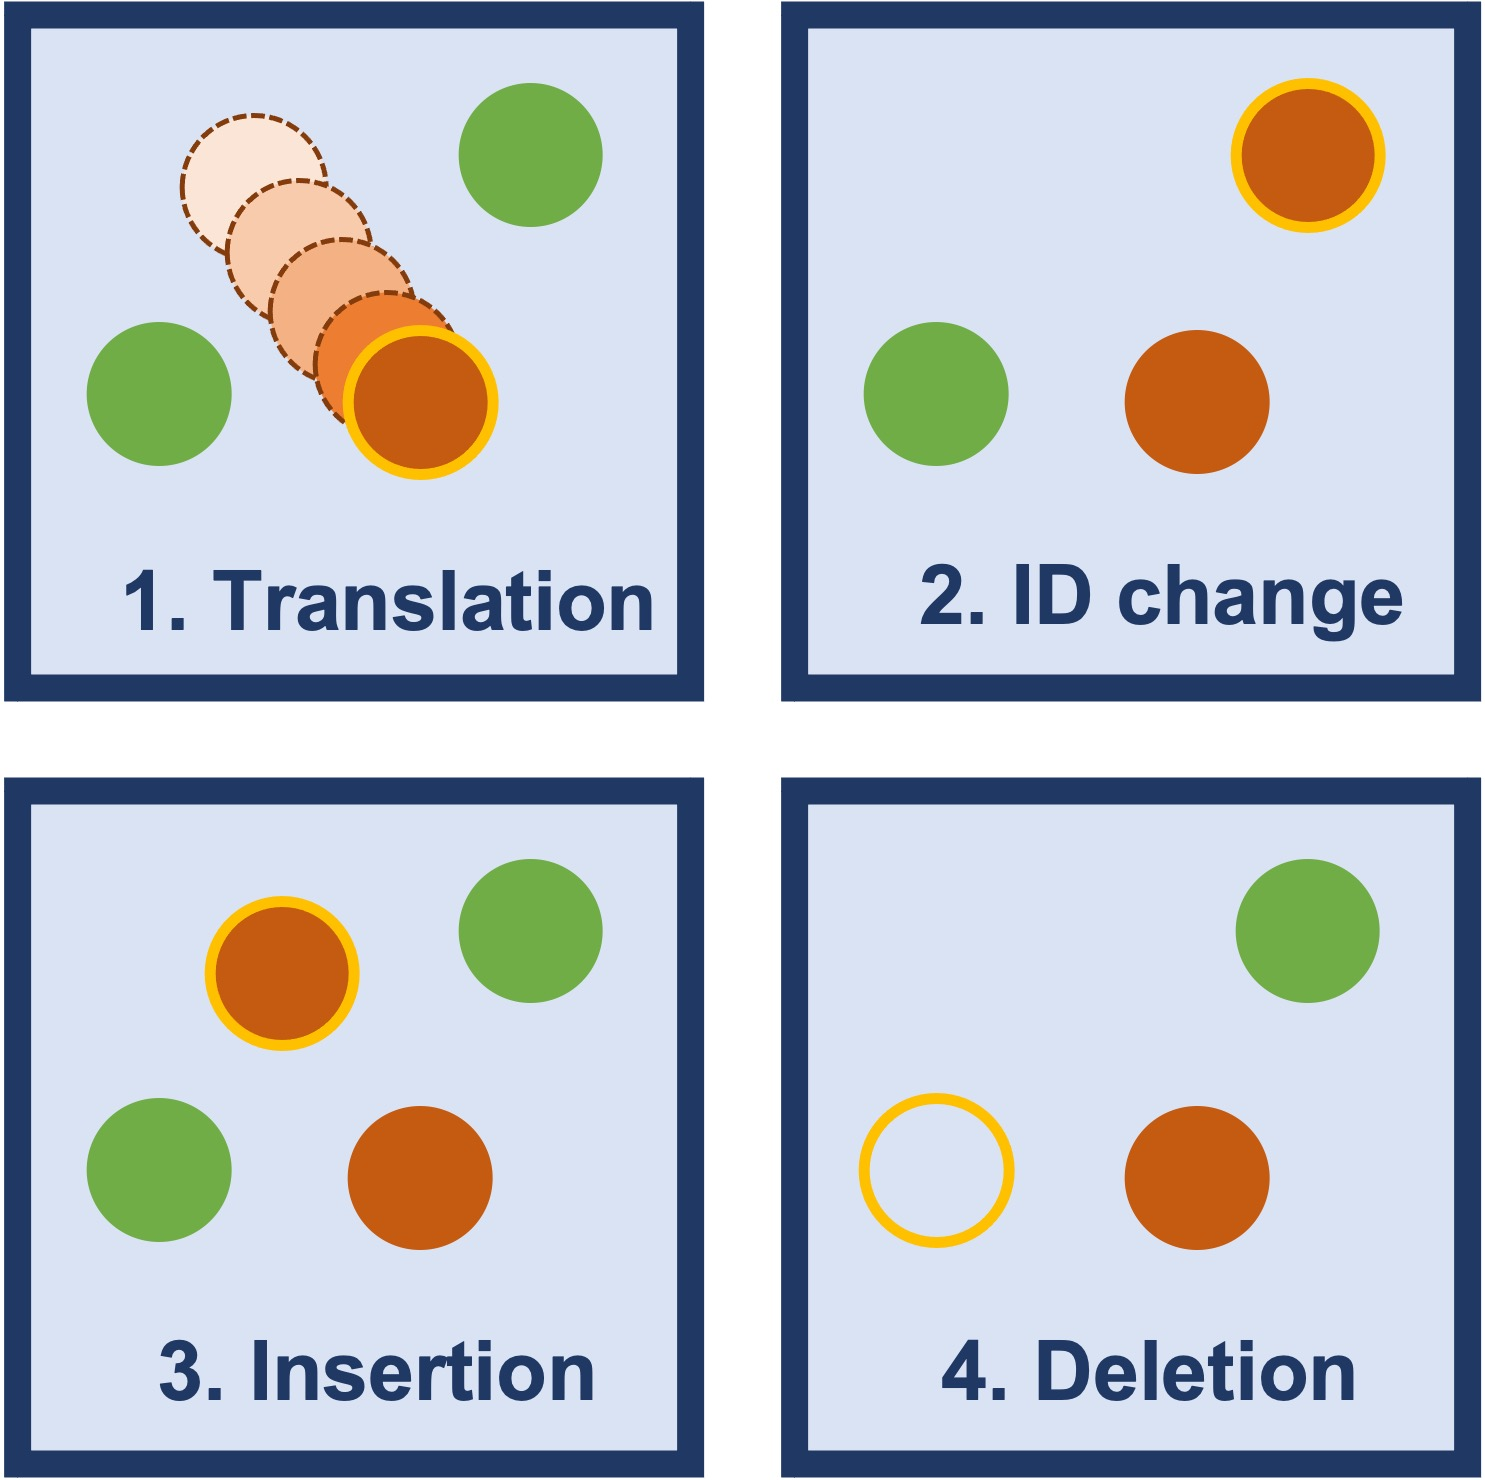
\includegraphics[width=0.99\textwidth]{figures/2-thermo/MC_moves.jpg}
  \caption{MC moves for monoatomic atoms with multiple components}
  \label{fgr:mc}
\end{figure}

To complete the description of the grand canonical Monte Carlo (GCMC) simulation we are interested in, let us now consider the different MC moves used to generate a configuraiton from another. Depending on the parameterization, these moves have different probabilities of occuring. For monoatomic atoms only four moves are relevant (see Figure~/ref{fgr:mc}): (1) the translation of a randomly chosen molecule with a displacement randomly chosen within a given radius, (2) the change of identity of a randomly chosen molecule into another, (3) the insertion of an adsorbate molecule and (4) the deletion of an adsorbate molecule. We deliberately omitted the rotations of the adsorbate because of the spherical symmtry of noble gases and the change of volume since the flexibility of the material framework is neglected. 

By using a GCMC algorithm, we can now generate a set of configurations according to their probability of occurence. Because the probability law is directly taken from equation \ref{eqn:gc}, the series of configurations describe the thermodynamic equilibrium state of a nanoporous material in contact with a reservoir of a xenon-krypton mixture at a given composition, pressure and temperature. Different thermdynamic quantities can be derived from ensemble averagings: the averaging loading or uptake at a given pressure (several pressures give the isotherm) and the isosteric heat of adsorption of each adsorbates (Xe and Kr). The ratio of the uptakes $q$ informs on the selectivity $s$ of the thermodynamic separation process: 
\begin{equation}
  s = \dfrac{q^{Xe}y^{Kr}}{q^{Kr}y^{Xe}}
\end{equation}
where $y^{Xe}$ and $y^{Kr}$ designate respectively the mole fractions of Xe and Kr in the gas phase reservoir.

To characterize a separation process, we theoretically only need to perform a GCMC calculation at every pressure conditions that we are interested in. However, this type of simulation requires a lot of time to converge since we need to test out a lot of insertion/deletion moves to accurately estimate the number of adsorbed molecules and the composition of the mixture. Hence, faster methods (machine learning) are developed to estimate the selectivity at any pressure conditions.\cite{Simon_2015,Kang_2023} If we are interested in the infinite dilution case, faster methods are already available, we are now going to introduce the Widom insertion that can estimate the adsorption performances at infinite dilution by estimating the Henry adsorption constant.  

\subsection{Widom insertion}

Widom insertion is not used to do this normally. Solvation enthalpy etc..

0-> 1 molecule can be used to estimate the free energy associated to the adsorption of a molecule at infinite dilution.


\section{Preliminary analyses}

As we have seen above in the existing literature, the computational screening of the nanoporous materials --- both existing frameworks and hypothetical structures --- for targeted adsorption properties has been the object of many studies, and several of those high-throughput screening studies have focused on noble gas separation, and Xe/Kr separation, in particular. For large-scale studies we have found that, in addition to the testing and validation of methodological developments, the screening aimed in most cases at one of three objectives: (i) to identify top performing materials for synthesis and/or characterization; (ii) to better understand the limits of possible performance, and the relationships and trade-offs between various metrics of performance (selectivity, uptake, etc); (iii) identify structure--property relationships, correlating separation performance with structural properties of the materials that can be more easily determined (i.e., at low computational cost).

\subsection{Thermodynamics of adsorption separation}\label{section:exchange}

Describe the interface. 

\todo{selectivity, entropy enthalpy, Henry coefficients}
difference between low pressure and higher pressure.

From microcanonical to Gibbs ensemble

\todo{Exchange equilibrium}

In order to analyze thoroughly the thermodynamics of competitive xenon and krypton adsorption using the results of both pure-component and multi-component GCMC simulations, we use in this work some thermodynamic properties (enthalpy and entropy in various conditions) associated with the following fictitious ``exchange equilibrium'':
\begin{equation} \label{eqn:exchange}
    \text{Xe}_{\text{(g)}} + \text{Kr}_{\text{(ads)}}
    \rightleftharpoons \text{Xe}_{\text{(ads)}} + \text{Kr}_{\text{(g)}}
\end{equation}
The equilibrium constant associated to the Equation (\ref{eqn:exchange}) at a pressure of 1\,atm for a given composition is simply the selectivity $s\e{1}$, defined above as a function of $y\ex{Xe}$, $y\ex{Kr}$, $q\ex{Xe}$ and $q\ex{Kr}$, respectively the mole fractions in the gas phase and the loadings in the material of xenon and krypton in the GCMC calculation. The enthalpy difference associated with this ``exchange'' equilibrium, $\Delta\e{exc}H\e{1} = \Delta\e{ads}H\e{1}\ex{Xe} - \Delta\e{ads}H\e{1}\ex{Kr}$, is defined as the difference of enthalpy between xenon and krypton within the mixture. Similarly, an entropy difference $\Delta\e{exc}S\e{1}$ can then be calculated as in Equation~\ref{eqn:entropy} (with $i = 1$):
\begin{equation} \label{eqn:entropy}
    \Delta\e{exc}S\e{i} = R\ln(s\e{i}) + \dfrac{1}{T}\Delta\e{exc}H\e{i}\ \ \ \mathrm{where}\ i\in\{0,1\}
\end{equation}

Furthermore, this ``exchange equilibrium'' can be generalized to the zero loading limit. A comparison of the thermodynamic quantities between the low pressure and ambient pressure cases is made possible by considering this equilibrium equation. The equilibrium constant at low pressure similarly corresponds to $s\e{0}$, the enthalpy to $\Delta\e{exc}H\e{0} = \Delta\e{ads}H\e{0}\ex{Xe} - \Delta\e{ads}H\e{0}\ex{Kr}$ and the entropy to $\Delta\e{exc}S\e{0}$ as written in Equation~\ref{eqn:entropy} (with $i = 0$).

The need of simul to find the optimal configuration. 


\subsection{Structure--selectivity relationships}

\todo{How SA VF and LCD are calculated}

\todo{Put analyses of selectivity relationship with other descriptors: uptake, void fraction, surface area, etc.}

\todo{Trade-offs etc. }

\begin{figure}[ht]
  \centering
  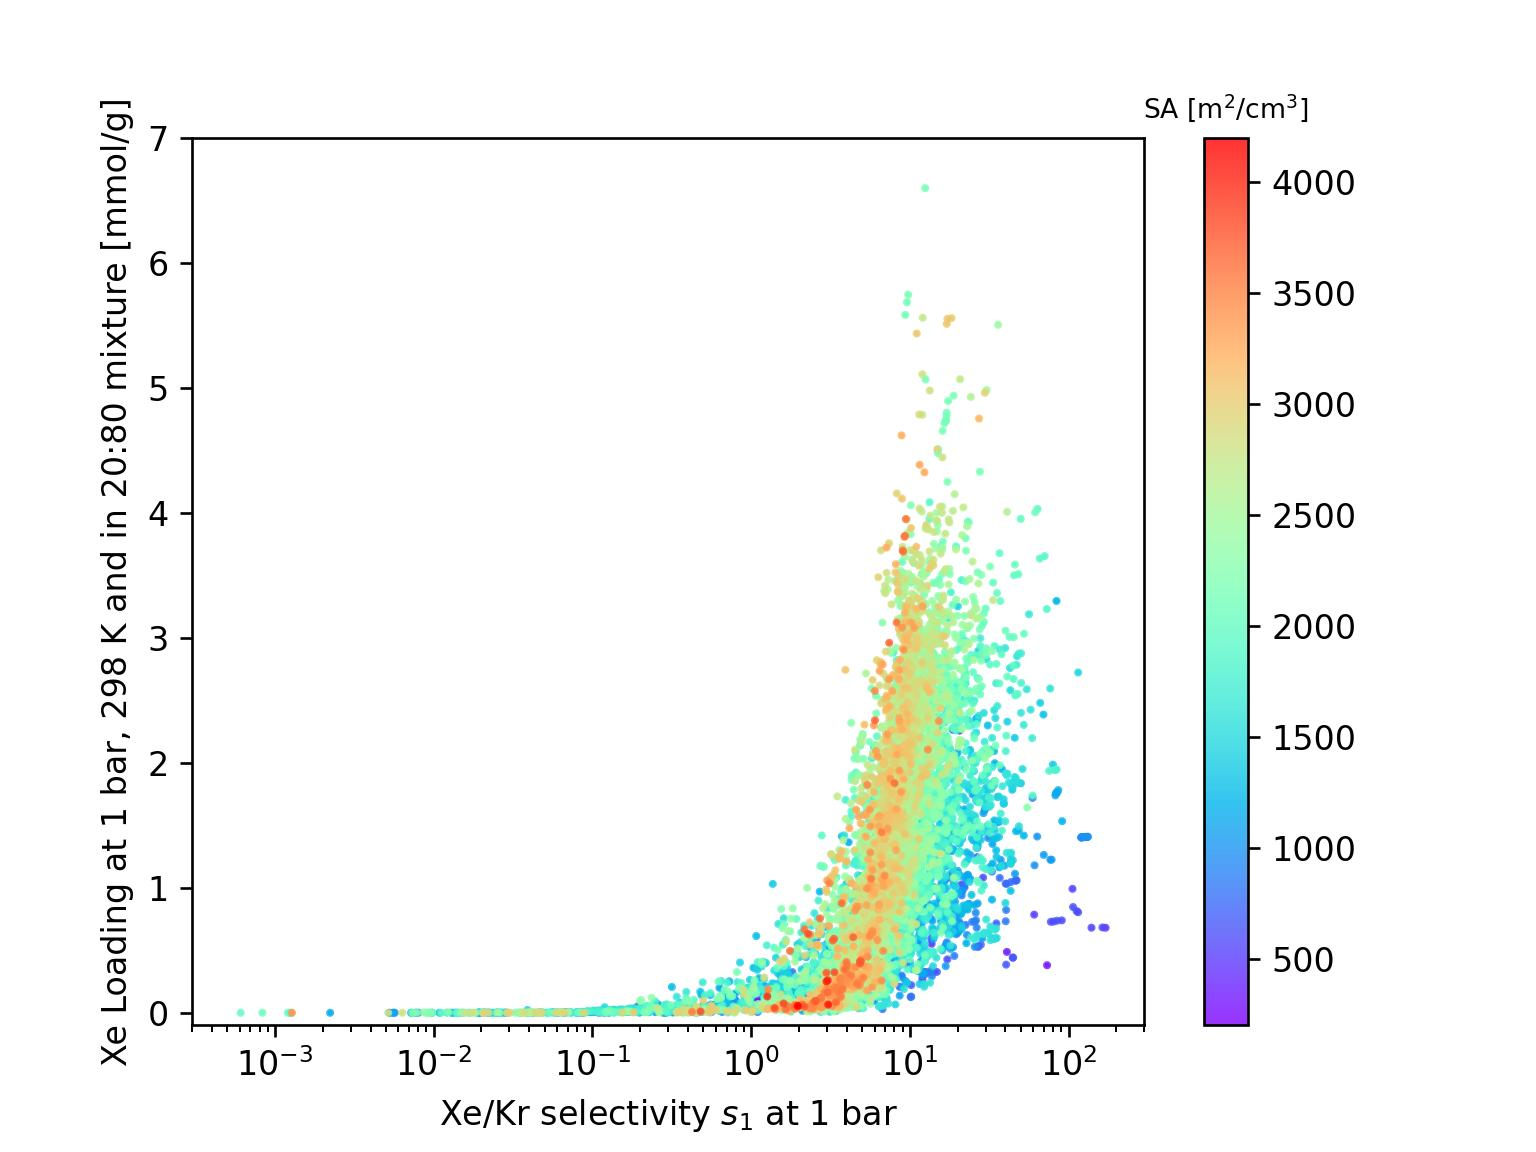
\includegraphics[width=0.48\textwidth]{figures/2-thermo/Scatterplot_uptake_selectivity_sa.jpg}
  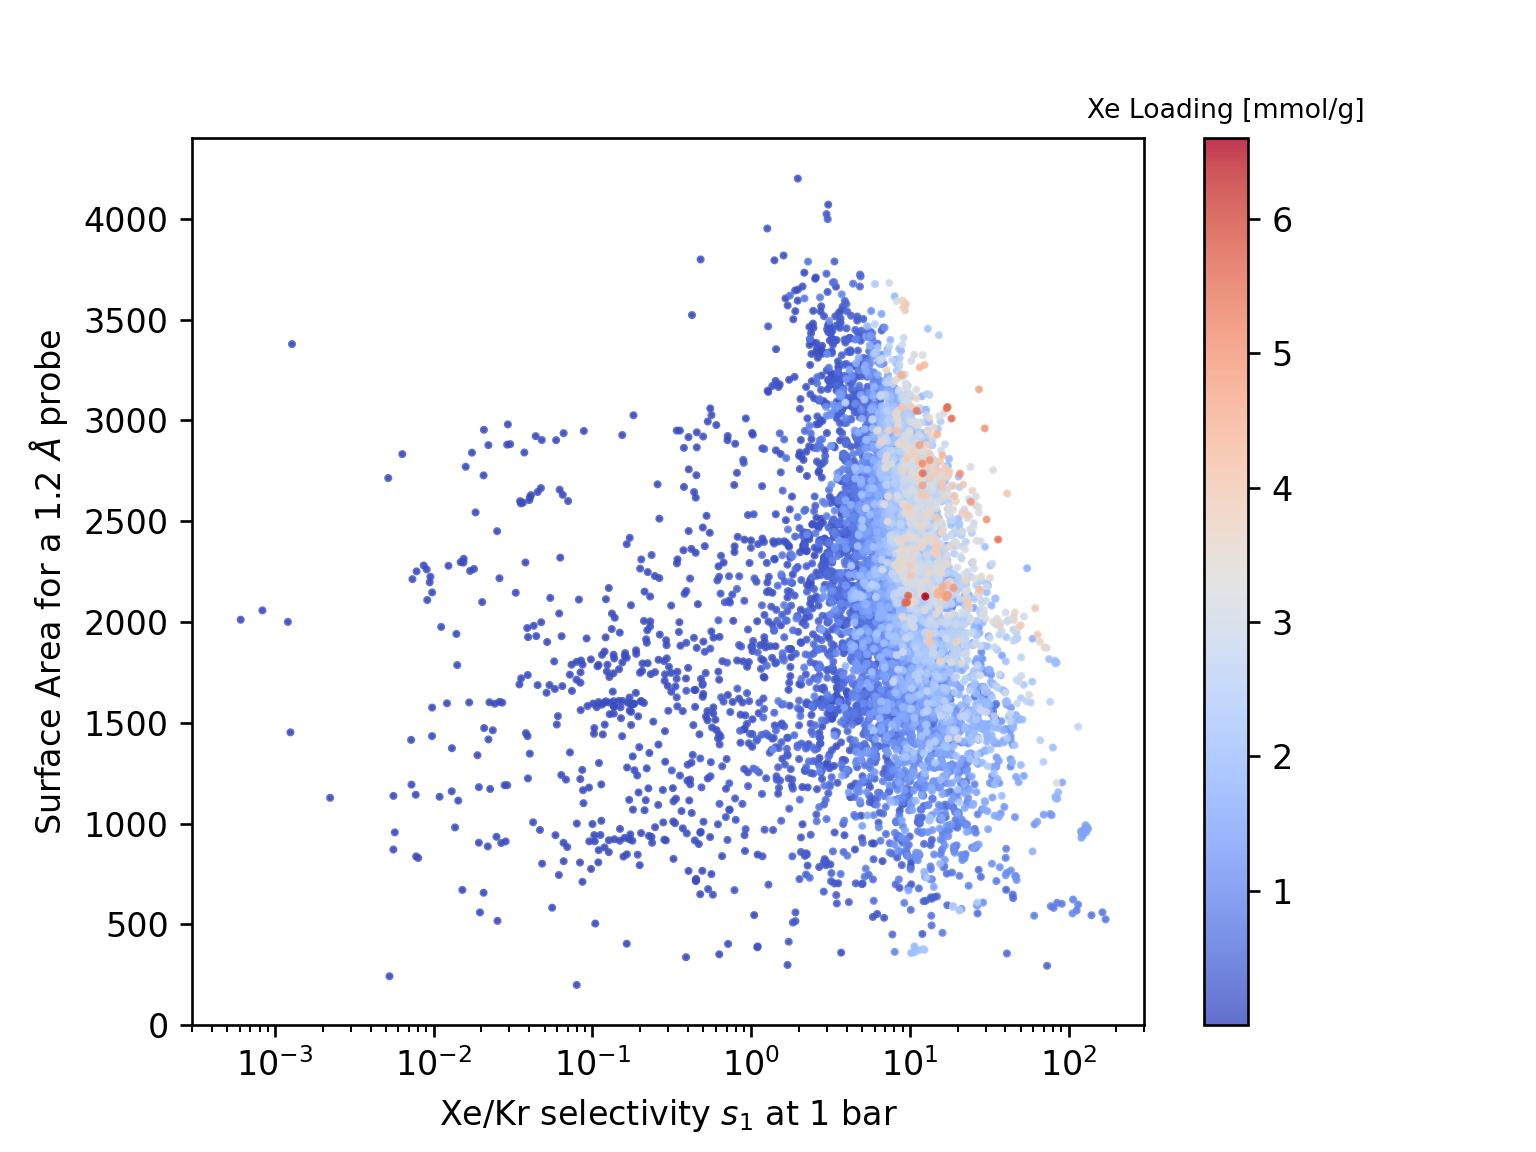
\includegraphics[width=0.48\textwidth]{figures/2-thermo/Scatterplot_sa_selectivity.jpg}
  \caption{Selectivity / Xe Uptake / Surface area}
\end{figure}

\begin{figure}[ht]
  \centering
  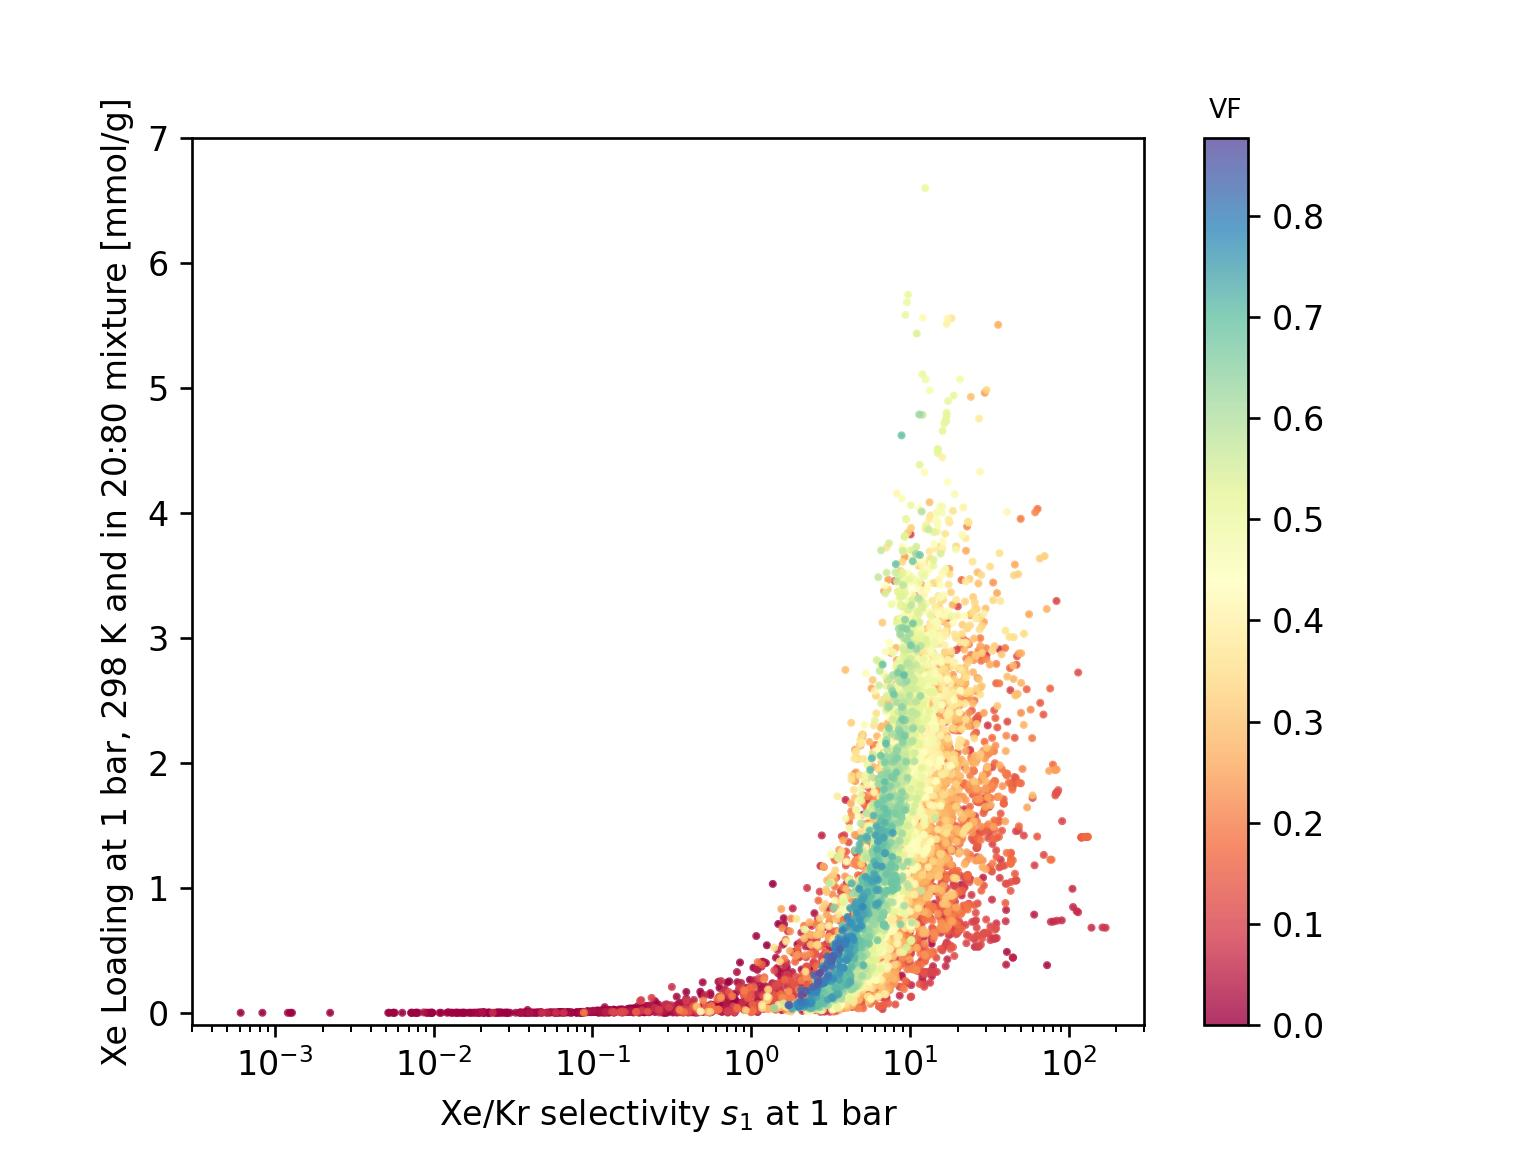
\includegraphics[width=0.48\textwidth]{figures/2-thermo/Scatterplot_uptake_selectivity_vol.jpg}
  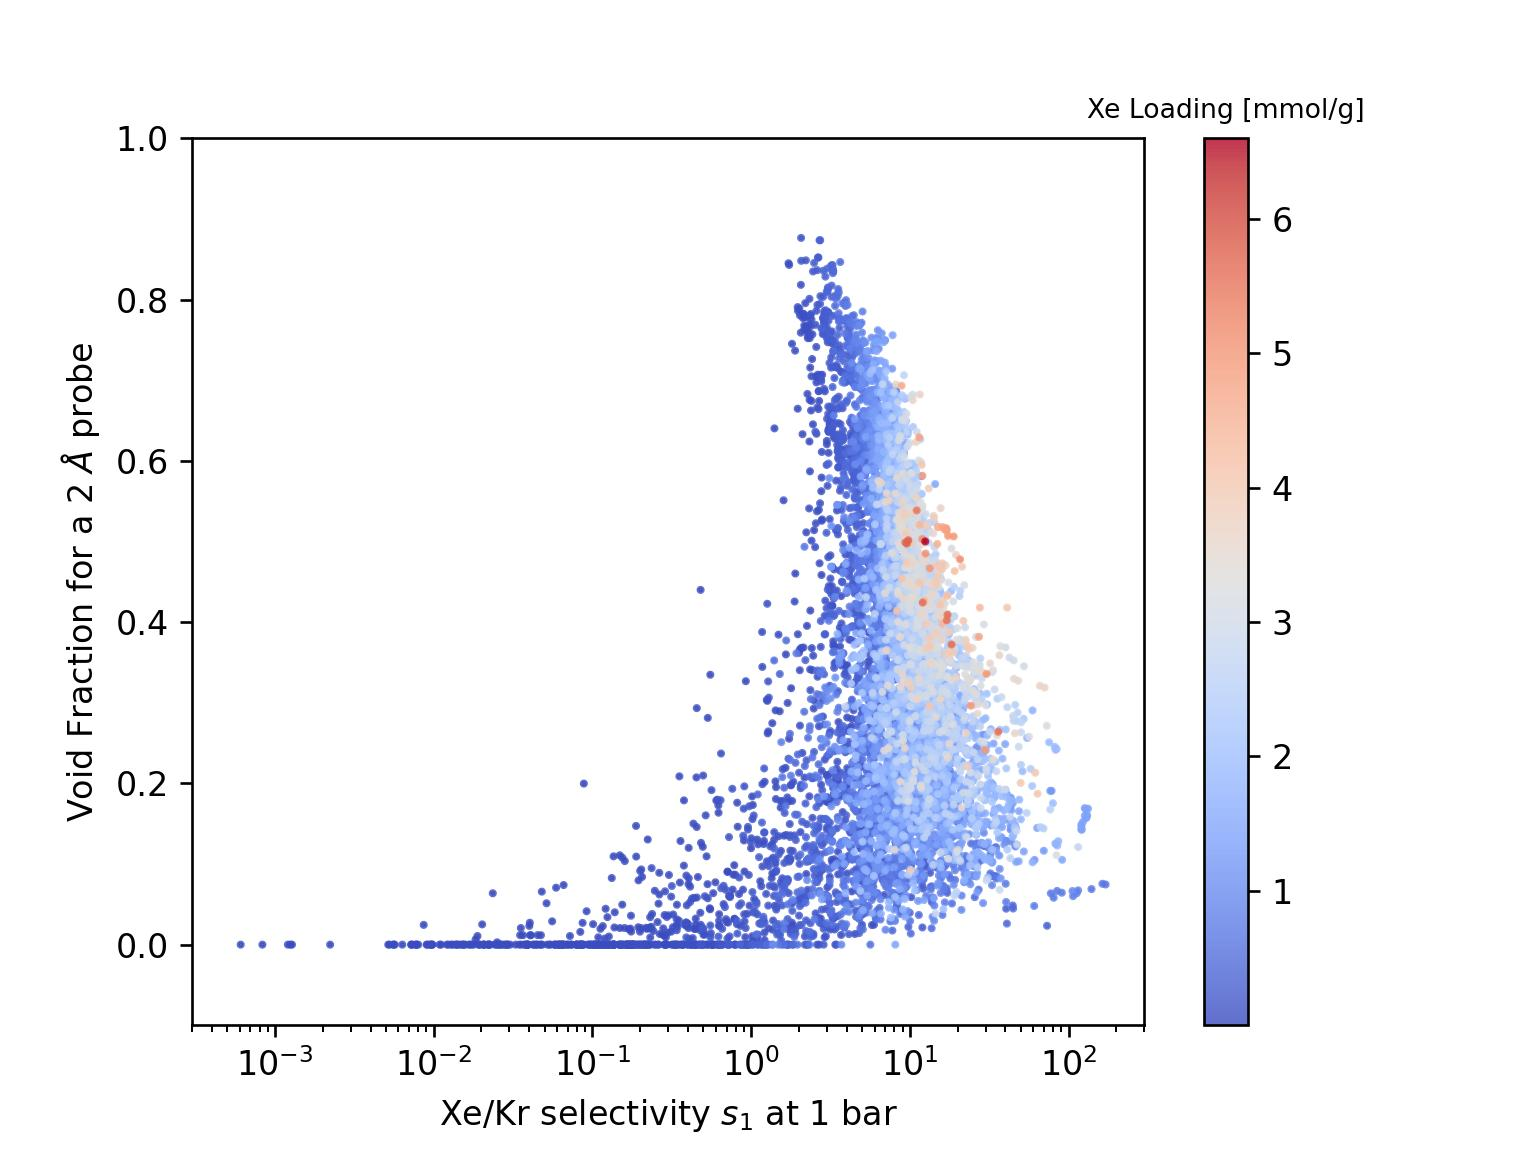
\includegraphics[width=0.48\textwidth]{figures/2-thermo/Scatterplot_vol_selectivity.jpg}
  \caption{Selectivity / Xe Uptake / Void Fraction}
\end{figure}


\begin{figure}[ht]
  \centering
  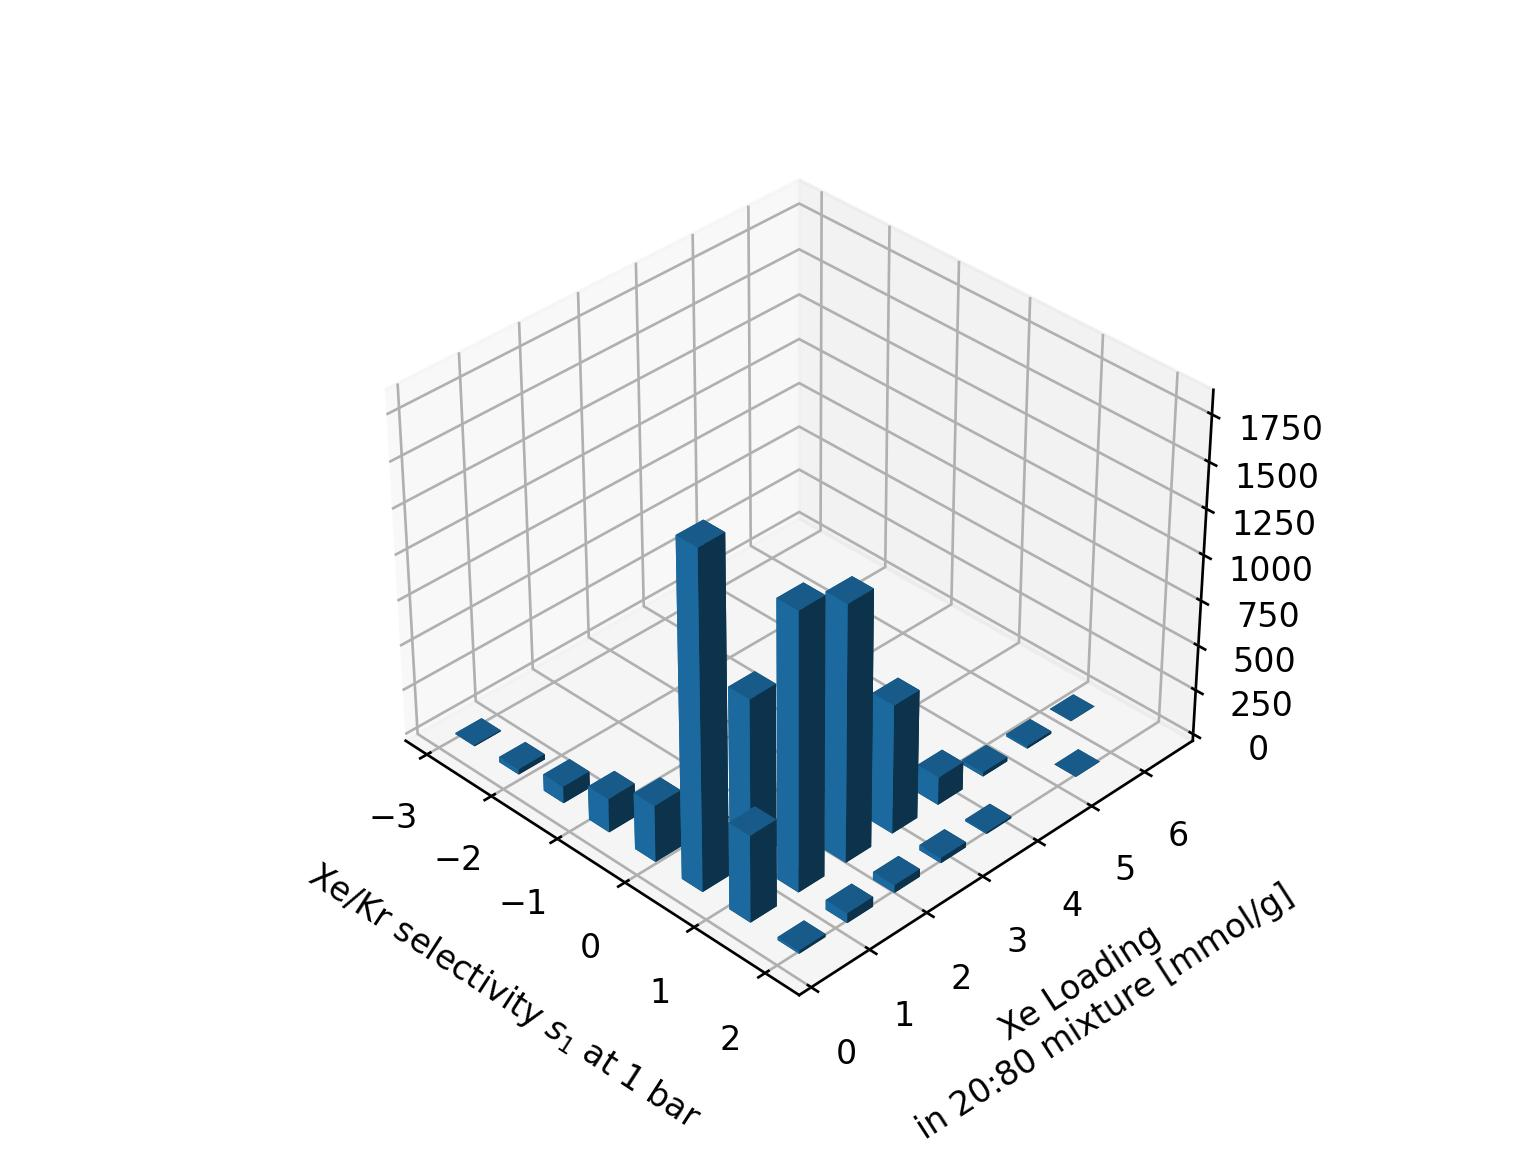
\includegraphics[width=0.7\textwidth]{figures/2-thermo/3D_hist_selec_uptake.jpg}
  \caption{Distribution selec / uptake}
\end{figure}

\begin{figure}[ht]
  \centering
  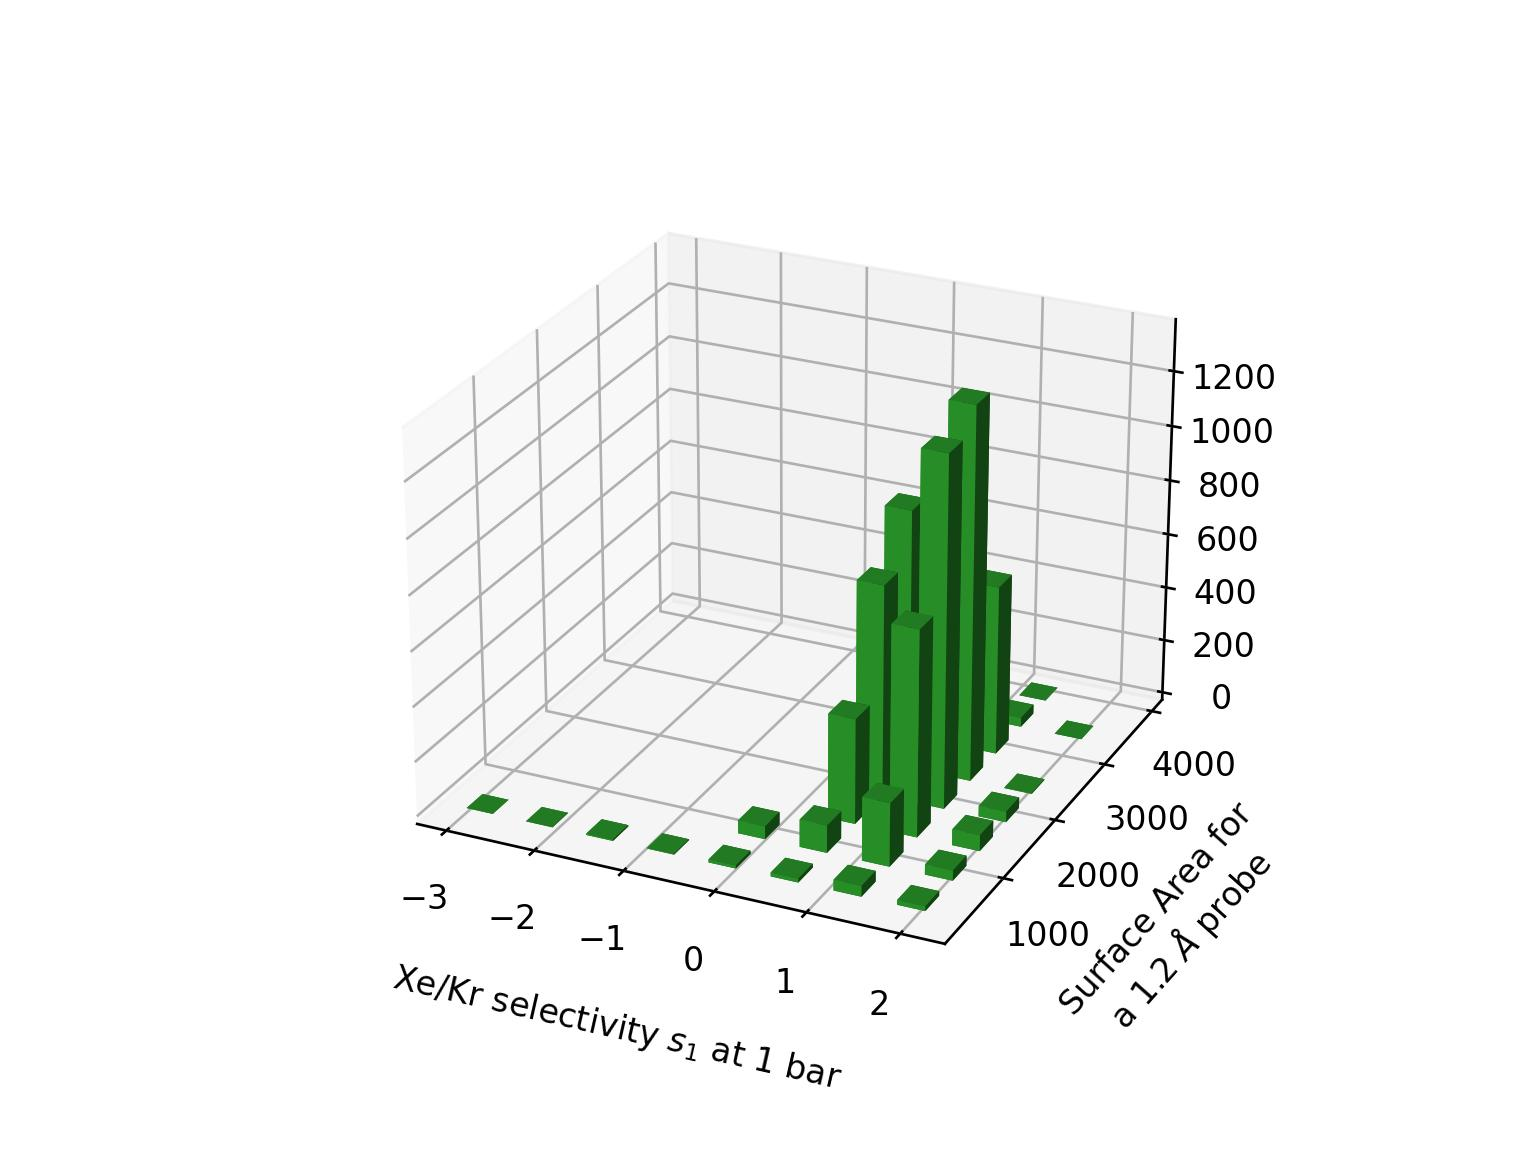
\includegraphics[width=0.48\textwidth]{figures/2-thermo/3D_hist_selec_SA.jpg}
  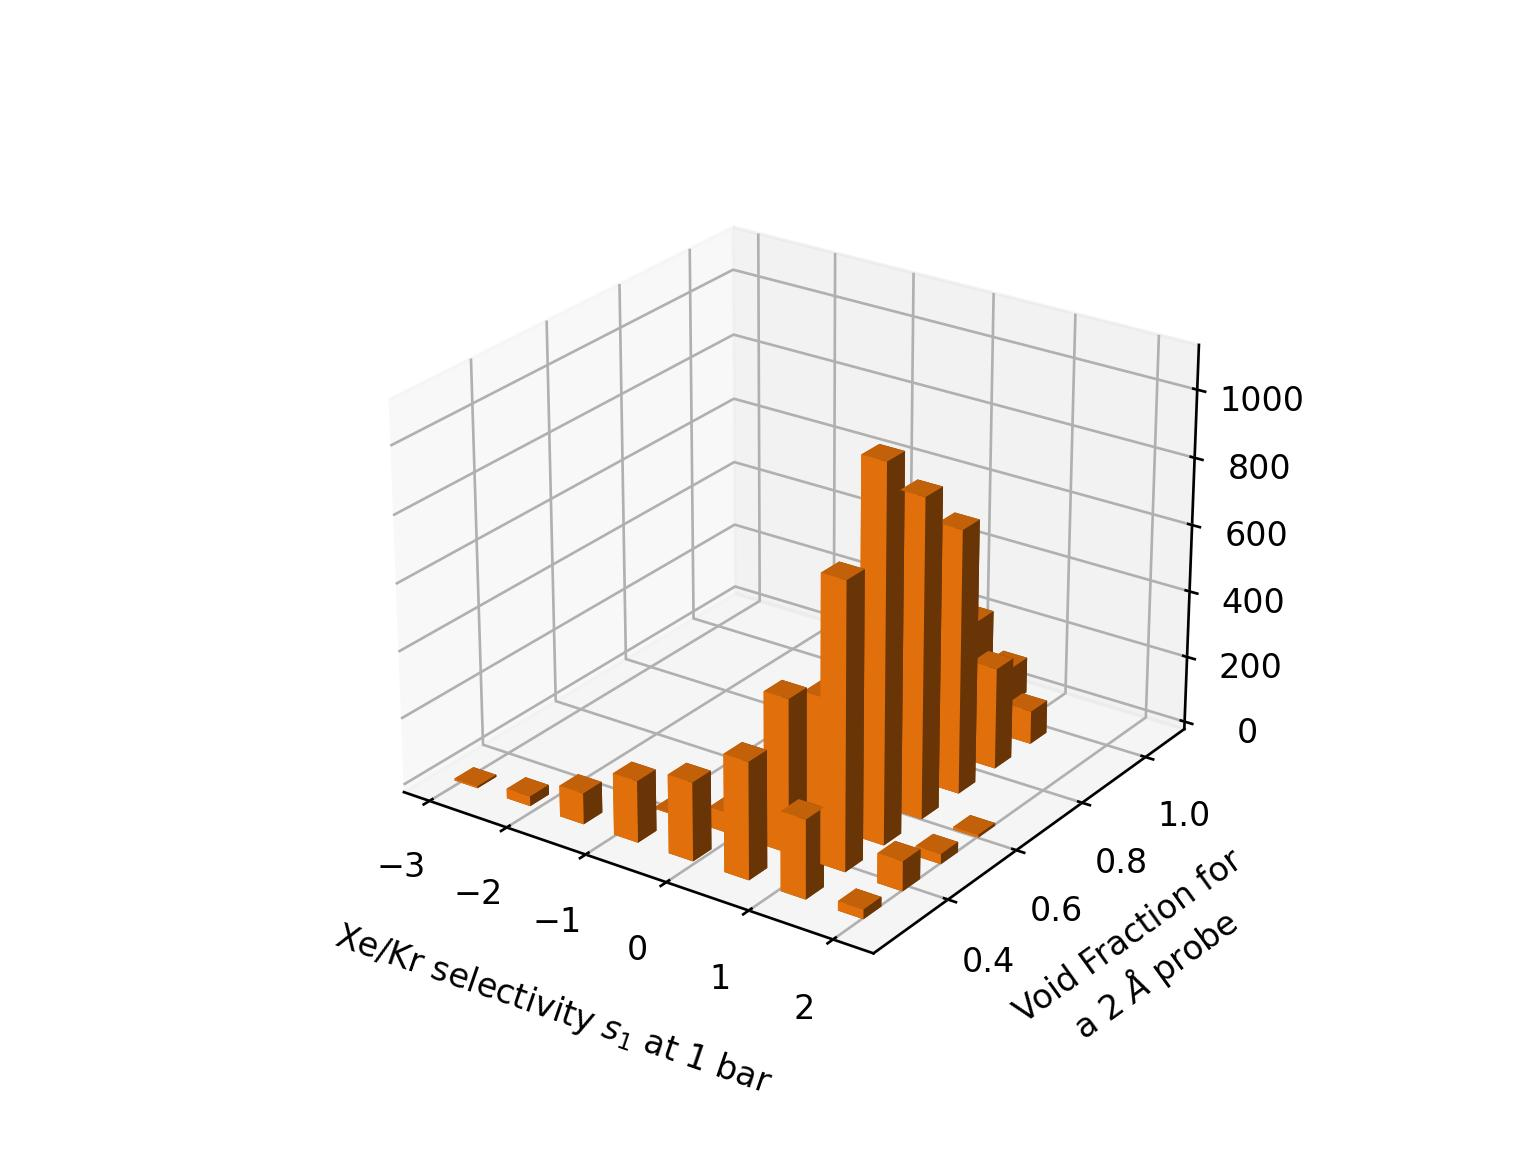
\includegraphics[width=0.48\textwidth]{figures/2-thermo/3D_hist_selec_vol.jpg}
  \caption{Ditributions, selec vs sa vol}
\end{figure}

\subsection{Thermodynamic quantities correlations}

In the present work, our goal is not directly to address the structure--property relationships, but rather to map out the details of the thermodynamic features of Xe/Kr adsorption and separation in nanoporous materials. We used the high-throughput screening methodology as a way to map out the space of thermodynamic properties, going beyond the usual quantities of selectivity and uptake, to focus more specifically on the role of adsorption enthalpy and entropy, the differences between Xe and Kr adsorption thermodynamics, and the differences between selectivity at low and high pressure.

To evaluate the performance of a given nanoporous material for separation in the low loading (or low pressure) limit, Henry's constants are often calculated from linear fits of low-pressure adsorption isotherm data --- both experimentally and computationally. In this section, we investigate the thermodynamics of Xe and Kr adsorption at low pressure. Here, We have calculated the low-pressure adsorption properties by using the Widom insertion method\cite{Widom1963, frenkel2001widom} on 9,668 structures from the dataset selected. It has higher accuracy than the fitting of isotherms, where it can be difficult to know what the extent of the linear adsorption regime is. With these simulations, we could obtain for each material the Henry's constant $K$ and the adsorption enthalpy $\Delta\e{ads}H\e{0}$ (at the zero loading limit) for both xenon and krypton. The Xe/Kr thermodynamic selectivity $s\e{0}$ in the low-pressure limit is then determined by the ratio $s\e{0} = K\ex{Xe}/K\ex{Kr}$ of the Henry's constants for the two gases. In the following, we look at the statistical relationships between the thermodynamic quantities at low pressure: $s\e{0}$, $K\ex{Xe}$, $K\ex{Kr}$, $\Delta\e{ads}H\e{0}\ex{Xe}$, $\Delta\e{ads}H\e{0}\ex{Kr}$ and $\Delta\e{exc}H\e{0}$ (which is defined in Section~\ref{section:exchange}).


\begin{figure}[t]
\centering
  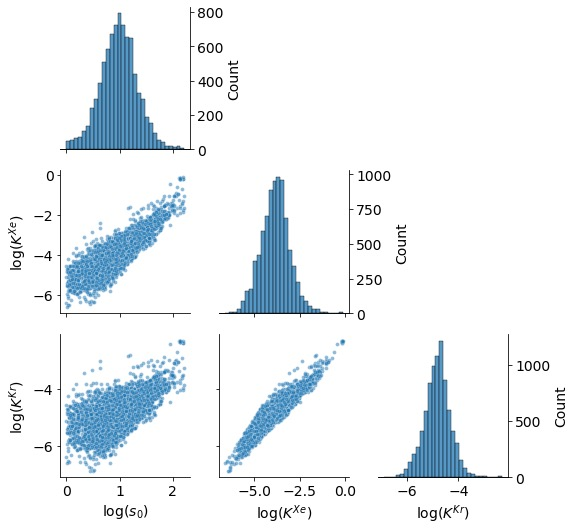
\includegraphics[width=\linewidth]{figures/2-thermo/Henry_0.jpg}
  \caption{\ For 8,401 MOFs with favorable thermodynamic Xe/Kr selectivity ($s\e{0} > 1$), pair-plots of $\log\e{10}(s\e{0})$, $\log\e{10}(K\ex{Xe})$ and $\log\e{10}(K\ex{Kr})$ (the Henry's constants are in \si{\milli\mol\per\gram\per\pascal}) in the off-diagonal subplots (note that the y-axis is displayed on the right side) and the distribution of each quantity are on the diagonal (note that the y-axis displayed on the right side corresponds to the count and the x-axis is correctly labeled below each subplot).}
  \label{fgr:histo_K}
\end{figure}


We display the distribution of thermodynamic properties of materials with favorable thermodynamic Xe/Kr selectivity ($s\e{0} > 1$) in Figure~\ref{fgr:histo_K} --- we restrict these plots to selectivity above 1, because those are the materials of interest for separation, and doing so removes several outliers with specific geometries or binding sites (but does not change the overall conclusions). We can first see that although the logarithm of the Xe Henry's constant $K\ex{Xe}$ is weakly correlated to the logarithm of the selectivity $s\e{0}$, this correlation is stronger for highly selective materials. Therefore, in a multistep screening study to identify the most selective materials, it could be possible to use as a ``first filter'' criterion based purely on Xe adsorption, discarding materials below a certain threshold (e.g., the materials with $s_0\ge30$ are contained in the subset with $K\ex{Xe}\ge2.7\,10^{-1}$~\si{\milli\mol\per\gram\per\pascal}). The correlation between $K\ex{Kr}$ and $s\e{0}$, on the other hand, is weaker.

With regard to Henry's constants, we observe a broad selection of behavior, with $K\ex{Xe}$ ranging from $2.6\ 10^{-7}$ \SI{}{\milli\mol\per\gram\per\pascal} to $7.9\ 10^{-1}$ \SI{}{\milli\mol\per\gram\per\pascal}, and $K\ex{Kr}$ ranging from $1.3\ 10^{-7}$ \SI{}{\milli\mol\per\gram\per\pascal} to $5.1\ 10^{-3}$ \SI{}{\milli\mol\per\gram\per\pascal}. We also see that statistically, a high affinity for xenon usually translates into a high (relative) affinity for krypton, which is a general trend for noble gases where the adsorption sites are not strongly specific. In order to look more in detail into the thermodynamics behind this wide diversity in behavior, we plot in Figure~\ref{fgr:histo_H} the enthalpies involved.


\begin{figure}[t]
\centering
  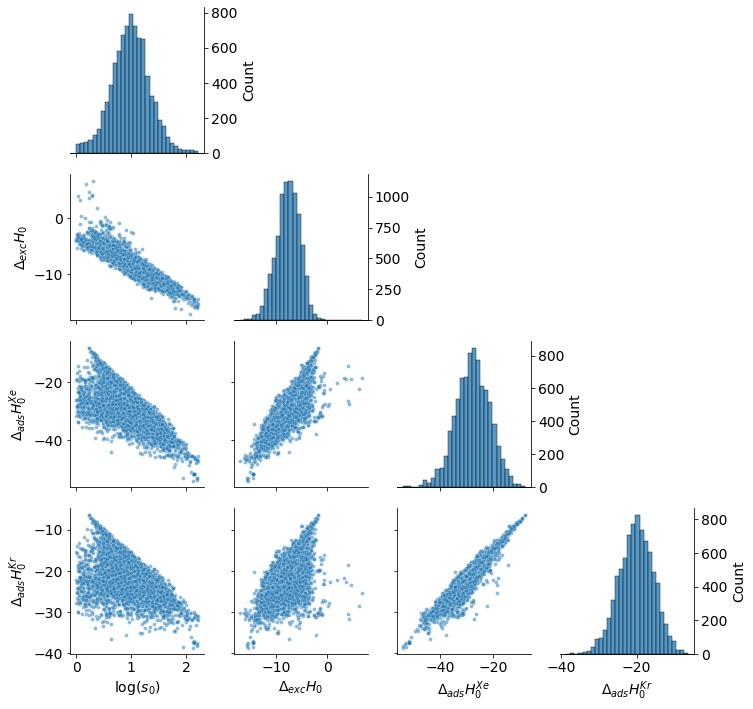
\includegraphics[width=\linewidth]{figures/2-thermo/Enthalpy_0_log.jpg}
  \caption{\ For 8,401 MOFs with favorable thermodynamic Xe/Kr selectivity ($s\e{0} > 1$), pair-plots of $\log(s\e{0})$, $\Delta\e{exc}H\e{0}$, $\Delta\e{ads}H\ex{Xe}\e{0}$ and $\Delta\e{ads}H\ex{Kr}\e{0}$ (the enthalpies are in \si{\kilo\joule\per\mol}) in the off-diagonal subplots and the distribution of each quantity are on the diagonal.}
  \label{fgr:histo_H}
\end{figure}

We first observe that the low-loading adsorption enthalpy of xenon ($\Delta\e{ads}H\ex{Xe}\e{0}$) is strongly correlated to that of krypton ($\Delta\e{ads}H\ex{Kr}\e{0}$). Echoing the similar correlation seen between respective Henry's constants, it suggests a rather generic physisorption mechanism is at play in the majority of materials, and that host--adsorbate affinities are mainly determined by the enthalpy. The main driver of Xe/Kr selectivity is neither the xenon or krypton adsorption enthalpy alone (both are weakly correlated to the selectivity), but as expected their difference, $\Delta\e{exc}H\e{0}$, which is strongly correlated to $\log(s\e{0})$. This is further confirmed by the lack of correlation between selectivity and adsorption entropies (\emph{c.f.} supplementary information, Figure~S2): the separation is mostly enthalpic in nature, and the entropy causes the dispersion in the correlation between selectivity $\log(s\e{0})$ and $\Delta\e{exc}H\e{0}$.

\section{Selectivity drop}

\subsection{Thermodynamic origins}\label{section:pressure}

\begin{figure}[t]
  \centering
    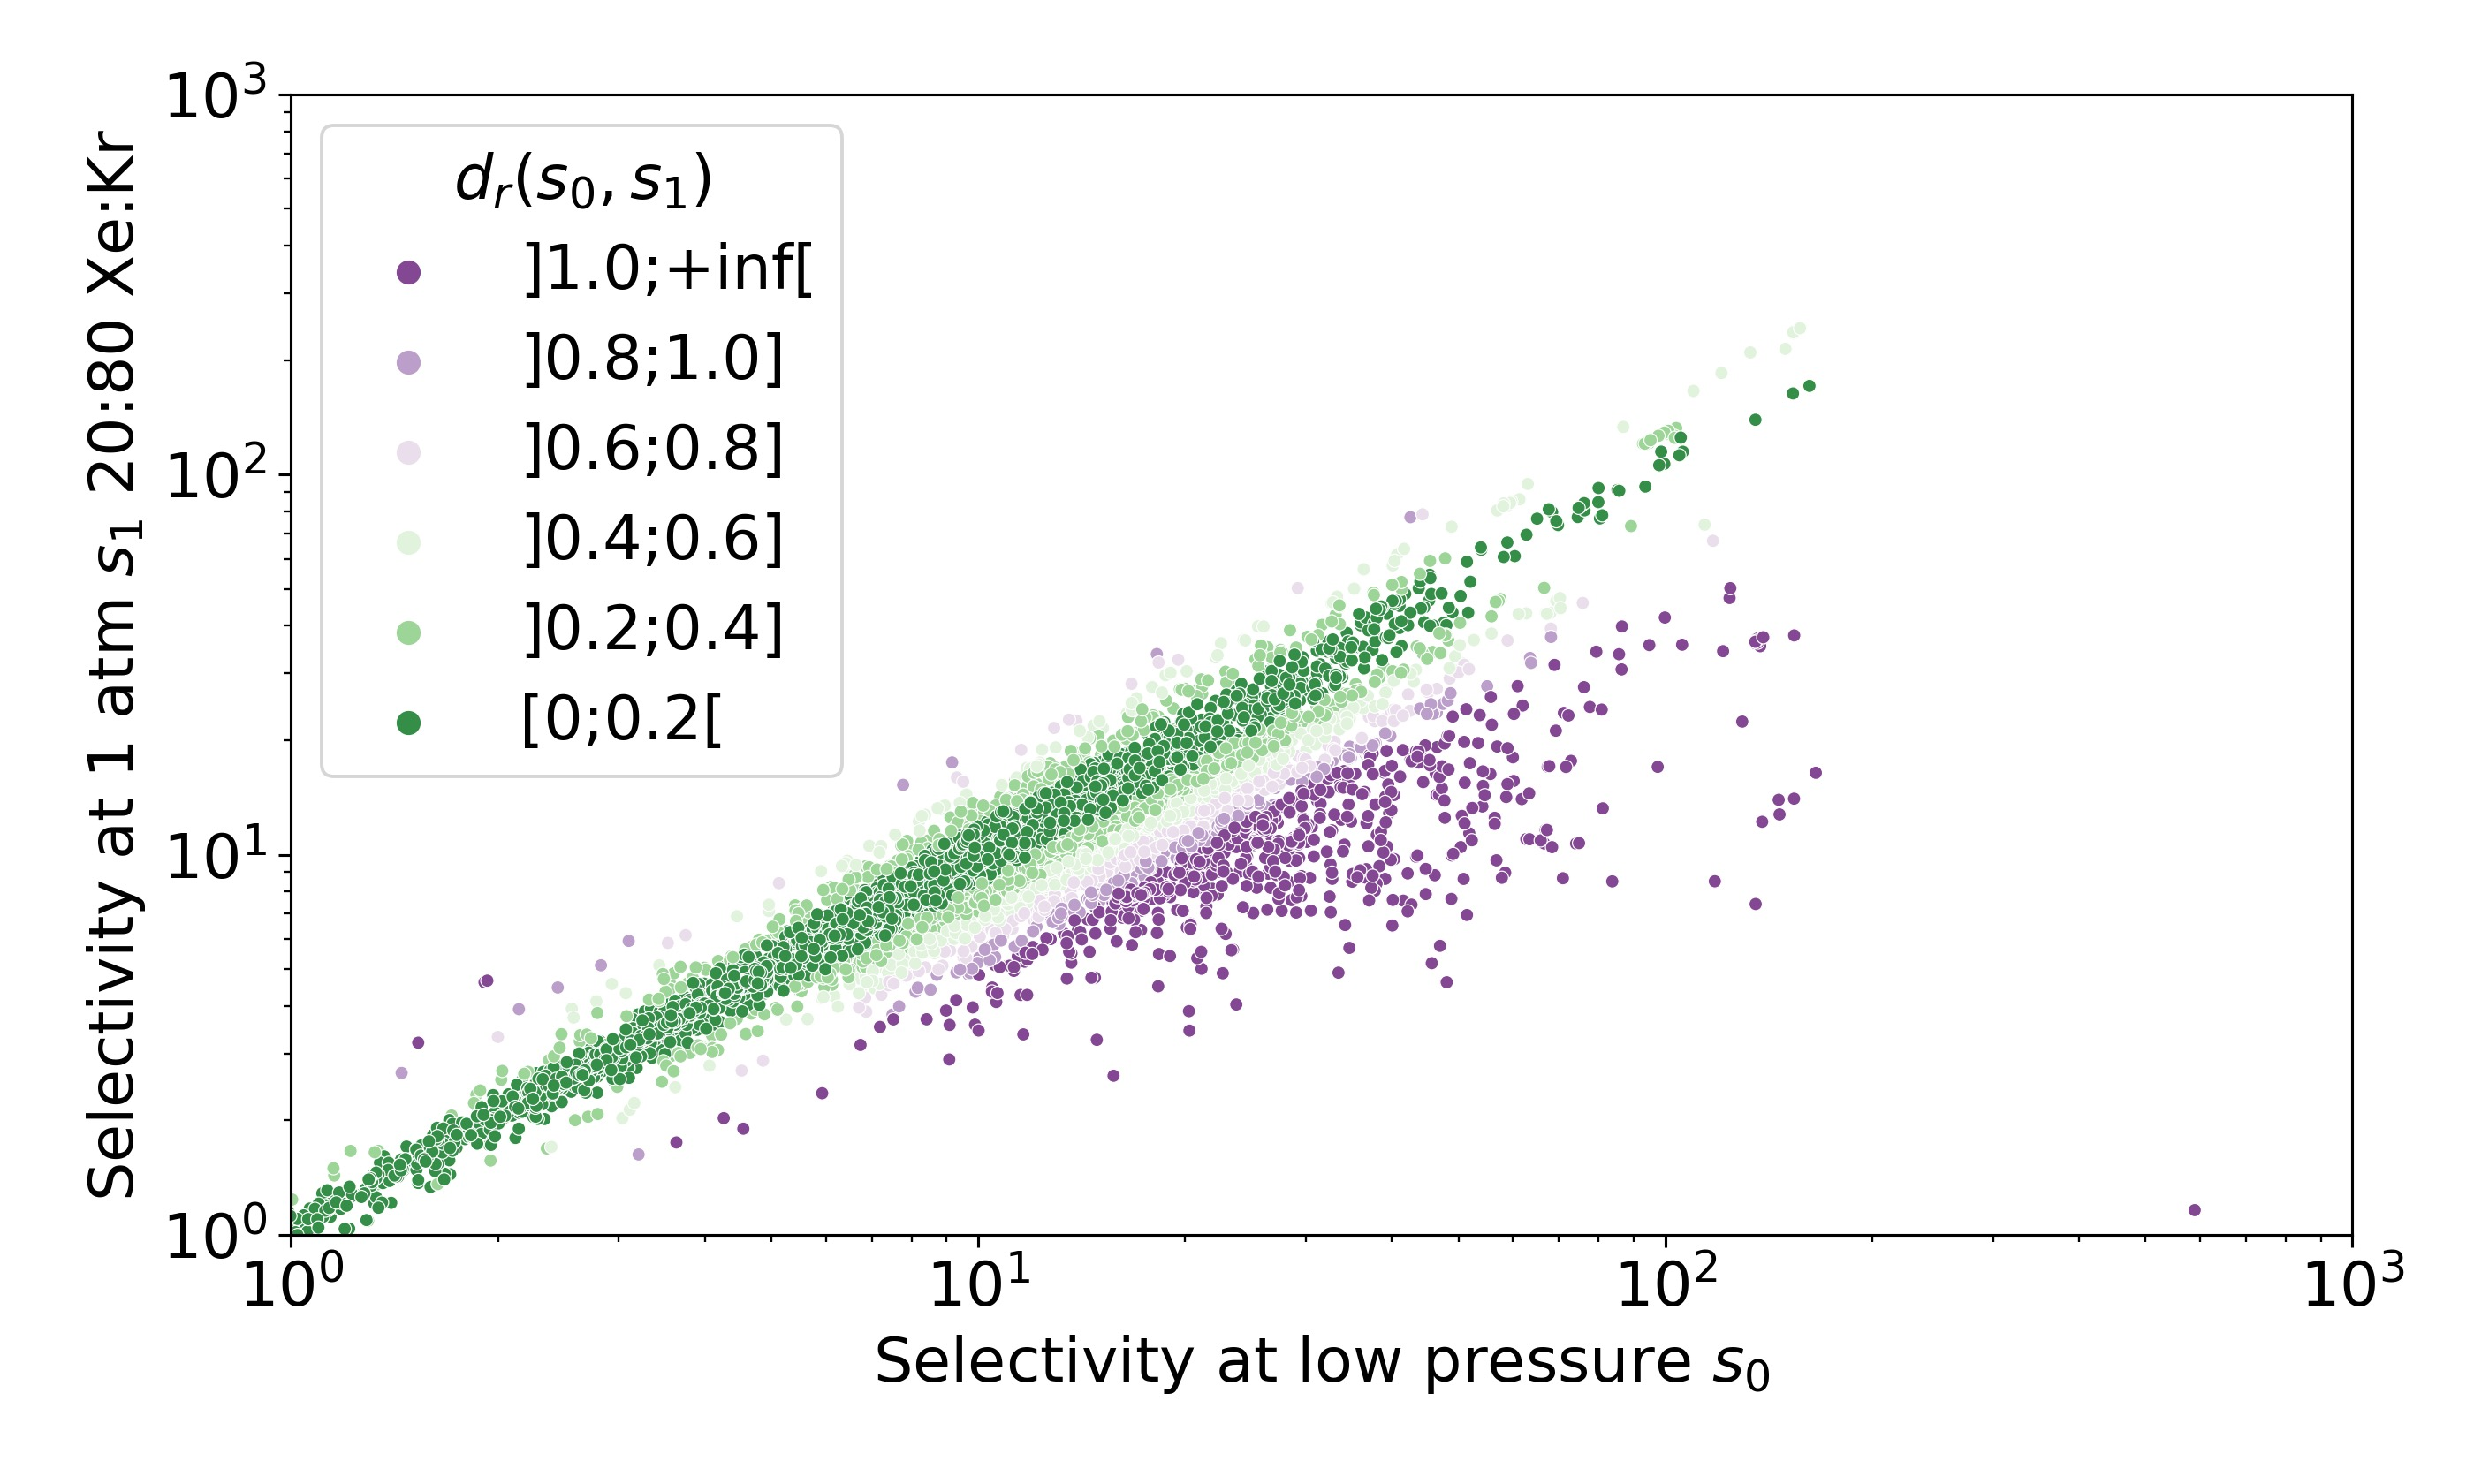
\includegraphics[width=\linewidth]{figures/2-thermo/s_0_vs_s_2080_overview_log.jpg}
    \caption{\ Difference of selectivity between low pressure and at a \SI{1013}{\hecto\pascal} pressure for a 20:80 xenon krypton composition. The relative difference between the low-pressure selectivity and the ambient-pressure is particularly high for the points labeled in purple.}
    \label{fgr:overview}
  \end{figure}
  
  In this section we focus on the impact of a change of working pressure on the adsorption selectivity, and analyze its thermodynamic origins. This is key to accurately assess the thermodynamics of adsorption in different working conditions for specific industrial processes, and any insight into the impact of pressure on selectivity may allow for faster screening limited at selected thermodynamic conditions.
  
  We calculated the selectivity $s\e{1}$ at pressure $1$~atm and ambient temperature using GCMC calculations on the entire dataset, with Xe/Kr mixture composition of 20:80 (found in a byproduct stream from air separation\cite{kerry2007industrial}) and 90:10 (found in the off-gas streams from nuclear waste\cite{auerbach2003handbook}). For high-selectivity materials, we find that the impact of composition appears rather marginal (\emph{c.f.} supplementary information, Figure~S5). In the following, we discuss the selectivity for the 20:80 mixture, which is the most commonly studied one in the literature. To measure the difference in selectivity between low and ambient pressures, we consider a relative difference $d_r(s\e{0},s\e{1})$ defined as follows:
  
  \begin{equation} \label{eqn:reldiff}
      d_r(s\e{0},s\e{1}) = \dfrac{\lvert s\e{0} - s\e{1} \rvert}{\min(s\e{0},s\e{1})}
  \end{equation}
  
  In Figure \ref{fgr:overview}, the selectivity at ambient pressure $s\e{1}$ is plotted against its low-pressure counterpart $s\e{0}$ (for materials where $s\e{0} > 1$, as before). The points are color-coded according to the value of $d_r(s\e{0},s\e{1})$, in 6 discrete categories for the sake of clarity. There is some broad level of correlation, see near the diagonal with {61.5\%} of materials where the difference is below {20\%} (near the $s_0 = s_1$ line). We also see clearly that there are many more points ({74.3\%} among the materials with $d_r(s\e{0},s\e{1})\ge 0.2$) below the first bisector ($s_1 < s_0$) than above: for these materials the selectivity $s\e{1}$ at 1~atm is significantly lower than the one at low pressure $s\e{0}$.
  
  This drop in selectivity mainly concerns the materials with a relatively high selectivity $s\e{0} > 10$ (see Figure~\ref{fgr:overview}), and forewarns that considering solely pure-component Henry's constant (i.e. zero-pressure selectivity) for materials screening could be misleading in some cases. Although it is simpler and faster to calculate, those low-pressure results that can overestimate selectivity by more than {100\%} in a significant number of materials (646 out of 9,668 in our dataset). By using a thermodynamic approach, we now try to explain the reasons behind these shifts in selectivity.
  
  To evaluate quantitatively the thermodynamic effects at play in the competitive adsorption in different regimes, we consider thermodynamic properties of the following ``exchange equilibrium'':
  \[
      \text{Xe}\e{(g)} + \text{Kr}\e{(ads)}
      \rightleftharpoons \text{Xe}\e{(ads)} + \text{Kr}\e{(g)}
  \]
  as described in Section~\ref{section:exchange}. We plot in Figure~\ref{fgr:HSplot_0} the exchange entropy at low pressure (plotted as $T\Delta\e{exc}S\e{0}$) against the 
  exchange enthalpy $\Delta\e{exc}H\e{0}$. In this scatter plot, the points are color-coded according to the selectivity $s\e{0}$ (with discrete categories for the sake of clarity), which is related to the enthalpy and entropy through Equation~\ref{eqn:entropy} --- meaning iso-selectivity lines are parallel straight lines in this scatter plot.
  
  
  \begin{figure}[t]
  \centering
    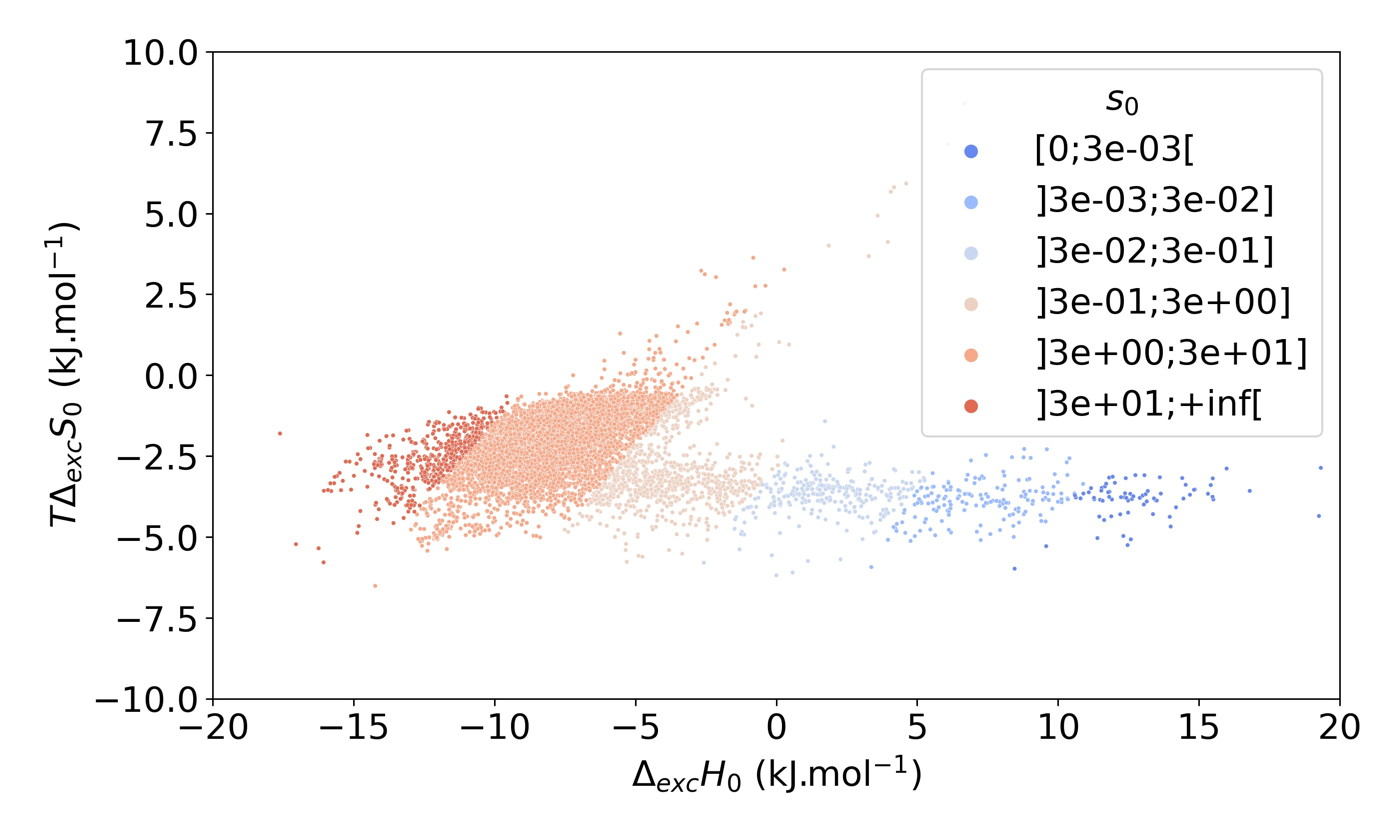
\includegraphics[width=\linewidth]{figures/2-thermo/enthalpy_entropy_0_s_0.jpg}
    \caption{\ The energetic equivalent of exchange entropy $T\Delta\e{exc}S\e{0}$ and enthalpy $\Delta\e{exc}H\e{0}$ at low pressure labeled using the selectivity $s\e{0}$ at low pressure. The limits between labels follows a affine function of slope $1/T$ and of intercept $-R\ln(s\e{0}\ex{lim})$ where $s\e{0}\ex{lim}$ is the limit selectivity value (\emph{cf.} Equation~(\ref{eqn:entropy})). In other words, the iso-selectivity lines are all parallel lines of equation $y=f(x)$ where $f$ is the affine function described previously.}
    \label{fgr:HSplot_0}
  \end{figure}
  
  
  \begin{figure}[t]
  \centering
    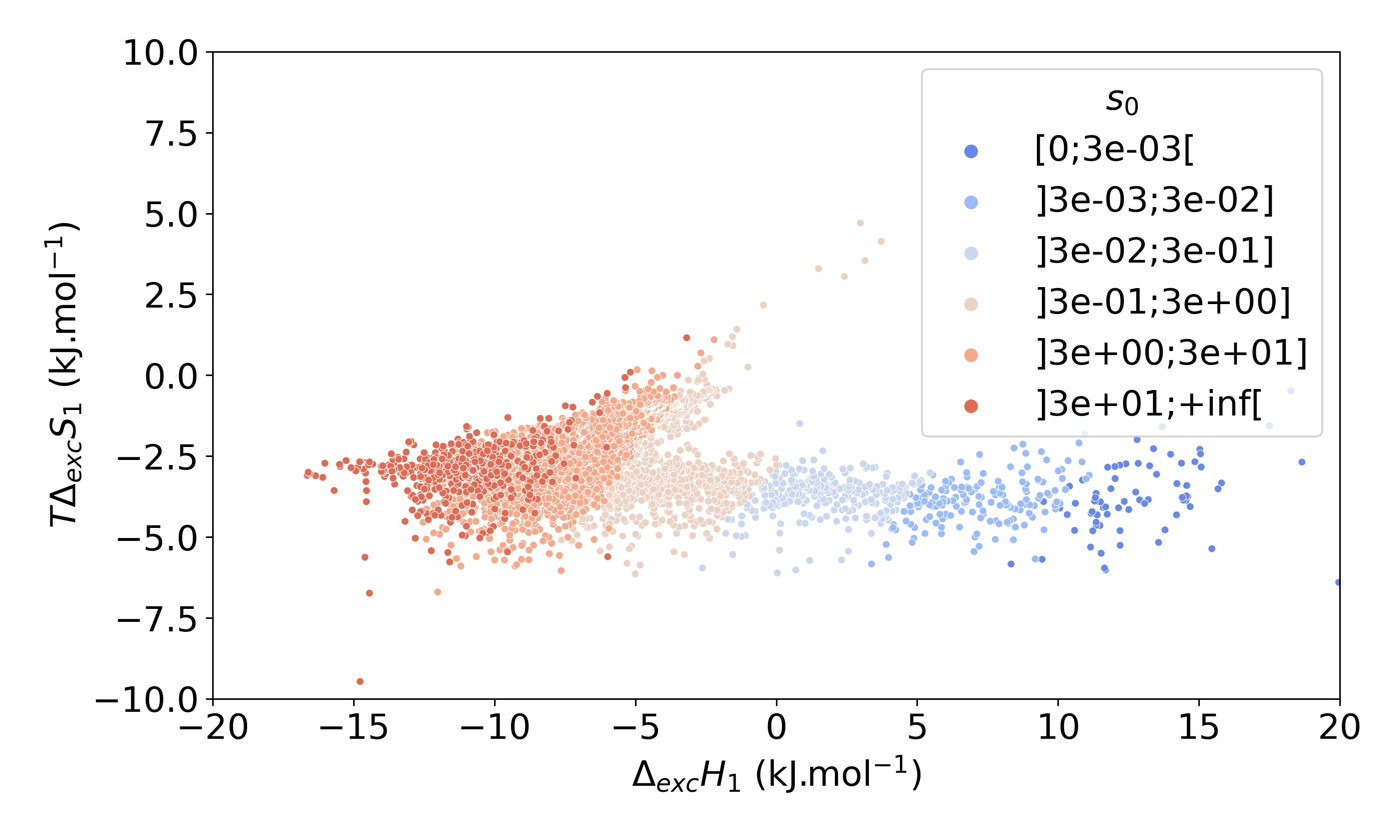
\includegraphics[width=\linewidth]{figures/2-thermo/enthalpy_entropy_2080_s_0.jpg}
    \caption{\ The energetic equivalent of exchange entropy $T\Delta\e{exc}S\e{1}$ and enthalpy $\Delta\e{exc}H\e{1}$ at ambient pressure labeled using the selectivity $s\e{0}$ at low pressure. The points are layered so that the points with higher $s\e{0}$ are always above. To see a split version of this plot, please refer to the Figure~S6 in the supplementary information.}
    \label{fgr:HSplot_1}
  \end{figure}
  
  
  In the supplementary information Figure~S8, we display the distributions of the exchange enthalpy and entropy at low pressure. For the 630 most selective materials ($s\e{0} > 30$), the distribution of the exchange enthalpy $\Delta\e{exc}H\e{0}$ is centered on $-12.0$\,\si{\kilo\joule\per\mol} with a standard deviation of $1.3$\,\si{\kilo\joule\per\mol}, whereas the distribution of the exchange entropy (plotted as $T\Delta\e{exc}S\e{0}$) is centered on $-2.5$\,\si{\kilo\joule\per\mol} with a standard deviation of $0.7$\,\si{\kilo\joule\per\mol}. These figures, along with the overall distribution plotted in Figure~\ref{fgr:HSplot_0}, further confirms the moderate role of entropy in the low-pressure selectivity: it is equivalent in average to about {20\%} of the exchange enthalpy at low pressure.
  
  Figure~\ref{fgr:HSplot_1} represents a scatter plot of the exchange entropy at $P = 1$\,atm $\Delta\e{exc}S\e{1}$ against the exchange enthalpy at ambient pressure $\Delta\e{exc}H\e{1}$. To compare it to the Fig.~\ref{fgr:HSplot_0}, the points are color-coded according to the low-pressure selectivity $s\e{0}$. Compared to the iso-selectivity $s\e{1}$ straight parallel lines (\emph{c.f.} supplementary information Figure~S7), we can see that many materials with high $s\e{0}$ have lower $s\e{1}$ --- seen as a migration of points to the right of the plot, compared to Fig.~\ref{fgr:HSplot_0}. This shift is therefore mainly due to a higher (less favorable) exchange enthalpy, hinting at an important role of enthalpy to determine higher pressure selectivity.
  
  To quantify this change, we consider the distributions of the exchange enthalpy $\Delta\e{exc}H\e{1}$ and the energetic equivalent of the exchange entropy $T\Delta\e{exc}S\e{1}$ at ambient pressure (Figures~S9). The enthalpy $\Delta\e{exc}H\e{1}$ is now centred on $-11.1$\,\si{\kilo\joule\per\mol} with a standard deviation of $1.9$\,\si{\kilo\joule\per\mol}. Compared to the zero-pressure values, the enthalpy distribution is more dispersed, showing that there are important changes in individual values, and is higher in average --- majority of materials have lower ambient pressure selectivity due to enthalpic effects. This can be explained by the very general increase of adsorption enthalpy upon loading in the gas phase, which is linked to the presence of more adsorbed molecules. In fact, the correlations (Figure \ref{fgr:histo_K}) suggest that highly selective materials have high affinity in xenon, therefore they feature significant uptake at 1\,atm and the large Xe loading means the most favorable adsorption sites can be saturated, and further adsorption involves weaker host--guest interactions and therefore increases the average adsorption enthalpy at nonzero loading.
  
  The entropic term $T\Delta\e{exc}S\e{1}$ is now centered on $-2.9$\,\si{\kilo\joule\per\mol}, with a standard deviation of $0.8$\,\si{\kilo\joule\per\mol} (almost unchanged from low-pressure). The entropy is on average lower, which means an overall less favorable separation due to entropic effects: this evolution of the entropic term hints at the potential of reorganization of the adsorbed molecules inside each material. The difference in distribution of enthalpy has, overall, more impact on the high-pressure selectivity than that of entropy. This suggests that the overall contribution of enthalpy remains more decisive than the role of entropy in the selectivity change, even at ambient pressure. This is an interesting conclusion for screening studies, because evaluation of adsorption enthalpy can be computationally faster than that of the adsorption free energy (or entropy).

\begin{figure*}[t]
  \centering
    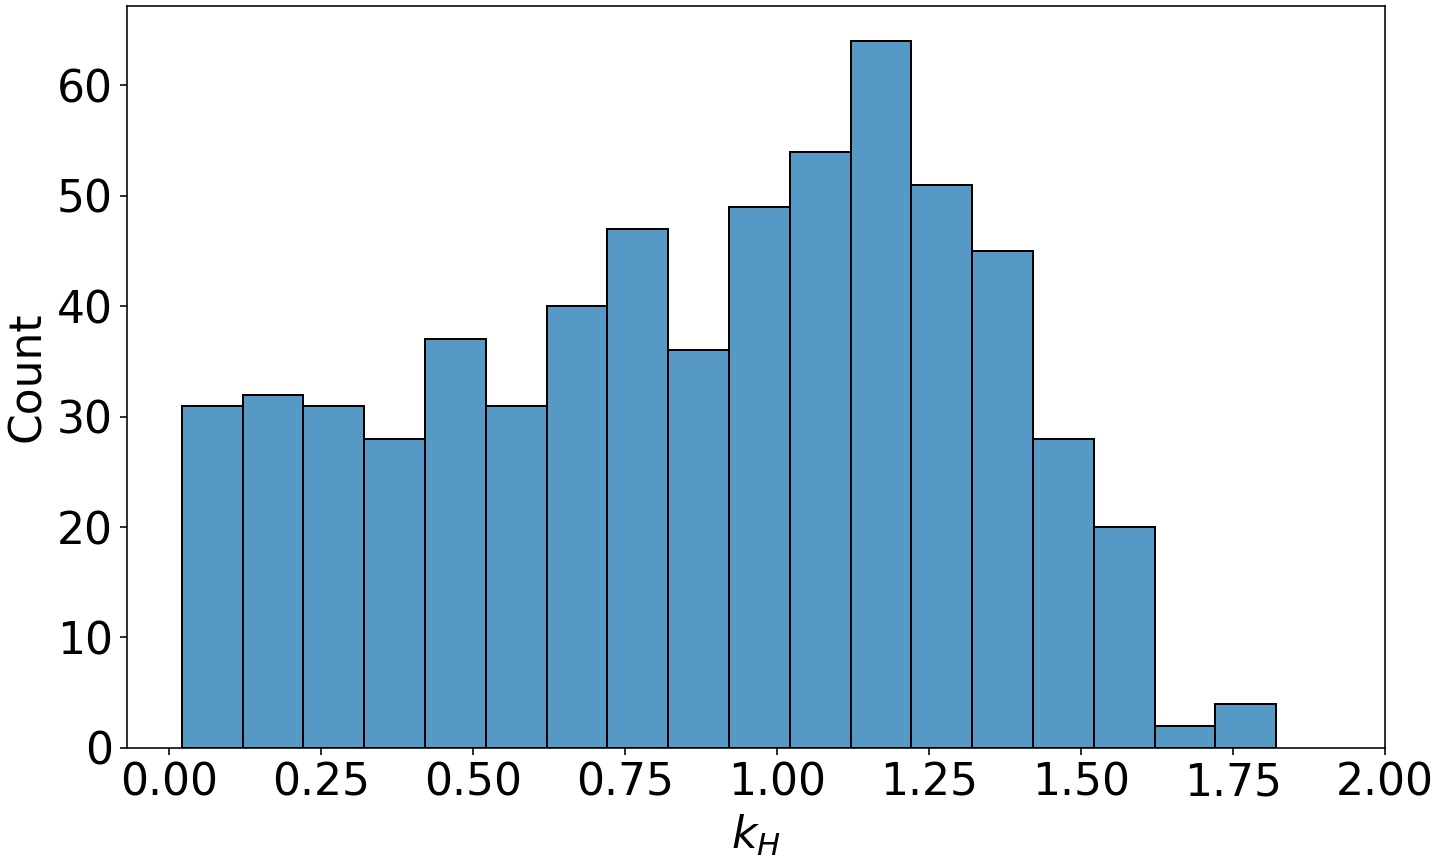
\includegraphics[width=0.37\textwidth]{figures/2-thermo/k_H.jpg}
    \hspace{8mm}
    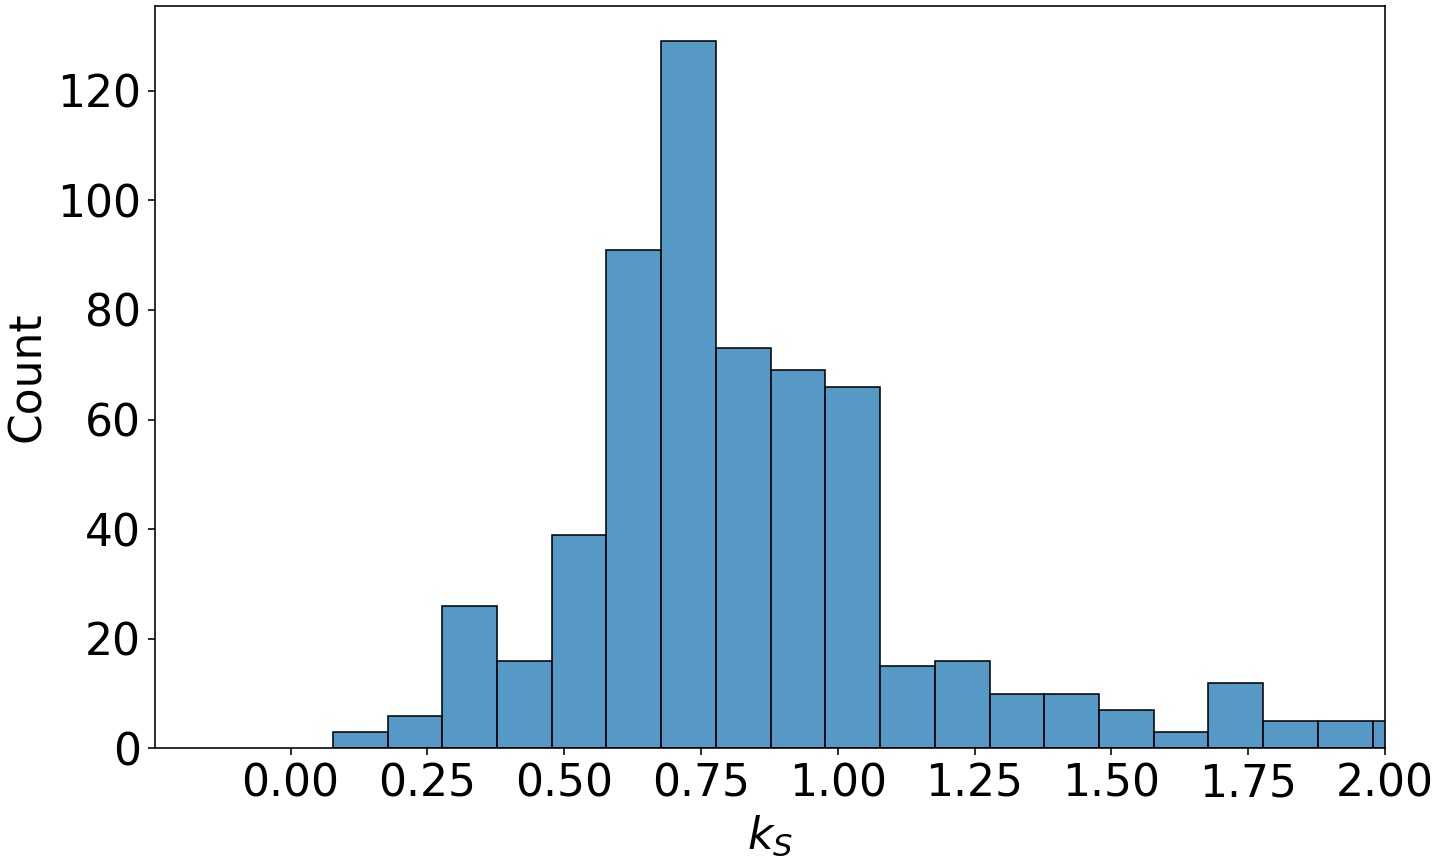
\includegraphics[width=0.37\textwidth]{figures/2-thermo/k_S.jpg}
    \caption{\ Distribution of the enthalpic $k\e{H}$ and entropic $k\e{S}$ contributions to the change of selectivity from low to ambient pressure for the 630 materials with $s\e{0}>30$. $k\e{H}$ has a rather uniform distribution, whereas $k\e{S}$ has a bell-like distribution. }
    \label{fgr:distk}
  \end{figure*}
  
  \begin{figure}[t]
  \centering
    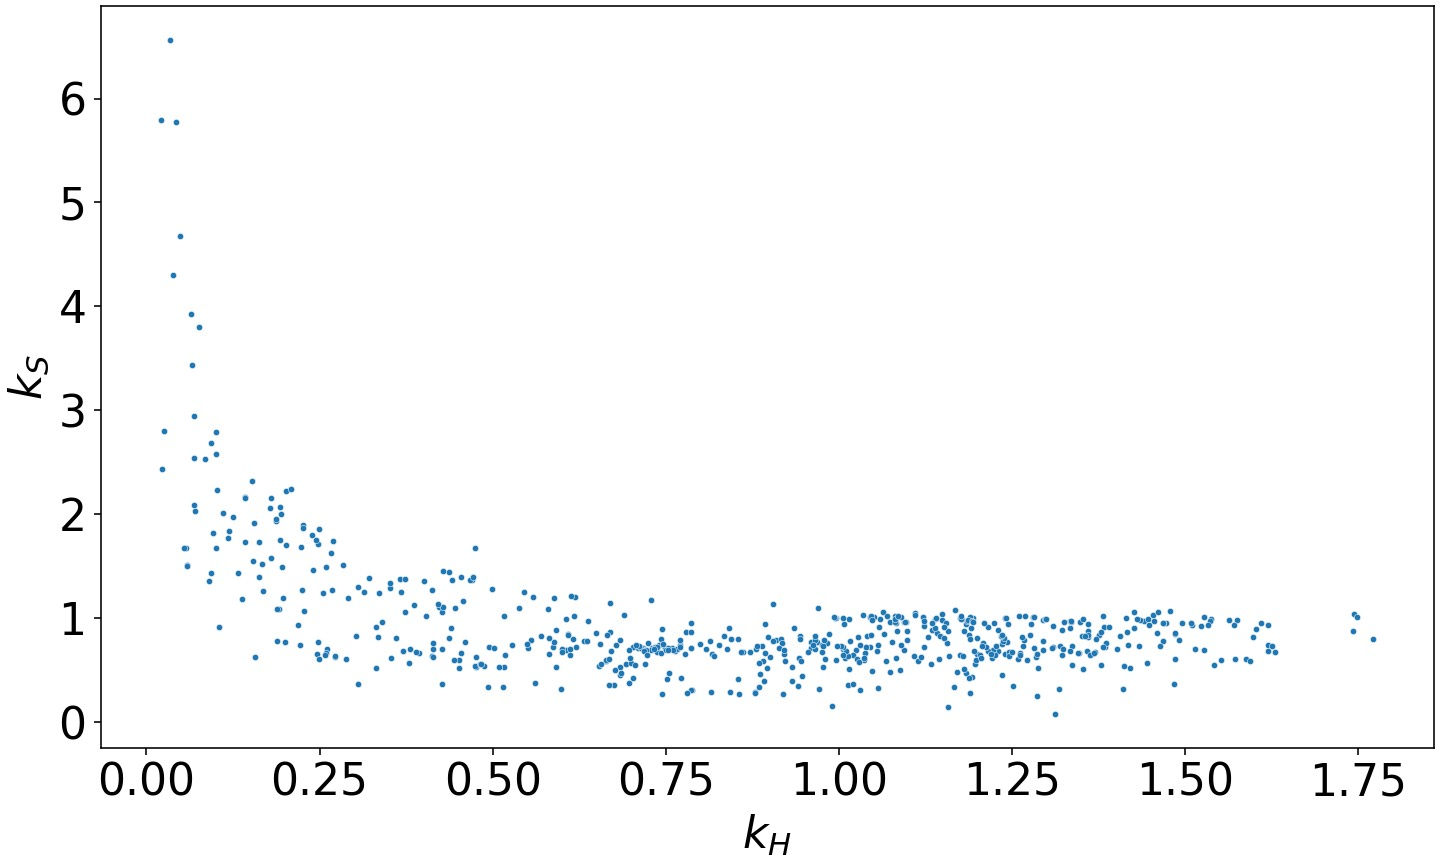
\includegraphics[width=0.45\textwidth]{figures/2-thermo/k_S_vs_k_H.jpg}
    \caption{\ Scatter plot of the enthalpic contribution $k\e{H}$ and entropic contribution $k\e{S}$ for the 630 materials with $s\e{0}>30$. The entropic compensation occurs when the enthalpic contribution is around $0.1$, else its value is around 1 and has little effect on the selectivity change.}
    \label{fgr:scatterk}
  \end{figure}
  
  To further investigate the thermodynamics of the selectivity change, we quantify in this section the contributions of enthalpy and entropy. The ratio ${s\e{1}}/{s\e{0}}$ is equal to the product $k\e{H} \times k\e{S}$ where $k\e{H}$ and $k\e{S}$ are the enthalpic and entropic contributions to the selectivity change defined as:
  \begin{equation}
  \label{eqn:effects}
      \begin{split}
       k\e{H} & = \exp\left(-\dfrac{\Delta\e{exc}H\e{1}-\Delta\e{exc}H\e{0}}{RT}\right) \\ k\e{S} & = \exp\left(\dfrac{\Delta\e{exc}S\e{1}-\Delta\e{exc}S\e{0}}{R}\right)
      \end{split}
  \end{equation}
  As we can see in Figure~\ref{fgr:distk}, the entropic contribution $k\e{S}$ has a bell-like distribution, with a mean of $0.9$ and a standard deviation of $0.6$. This confirms that $k\e{S}$ is close to $1$, and has therefore only a marginal effect on the selectivity change. On the other hand the enthalpic contribution $k\e{H}$ has a more uniform distribution ranging from $0.1$ to $1.5$, which means that enthalpy has a crucial role in the selectivity change we observe. There are a significant number of materials with a $k\e{H}$ close to zero, they correspond to the same materials highlighted in Section~\ref{section:pressure}.
  
  Furthermore, the scatter plot of $k\e{H}$ and $k\e{S}$ (shown in Figure~\ref{fgr:scatterk}) confirms a rather moderate effect of entropy. For most of the materials with $0.25 \le k\e{H} \le 1.75$, we see that $k\e{S}$ is close to 1. The most significant entropic contributions are found for materials where $k\e{H}$ is close to zero (typically below 0.25). If we look in more detail at the 29 materials with $k\e{S}>2$, the entropic contribution $k\e{S}$ moderately compensate the enthalpic contribution as the average ratio $s\e{1}/s\e{0}$ is around $0.25$. In such cases, the entropy is non-negligible and it can partially compensate the enthalpic contribution to the selectivity change, but the general trend is still given by enthalpy, since the overall selectivity is decreasing as a result.
  
  
  \subsection{Detailed investigation}
  \label{sec:archetypes}
  
  In this section, we go over some of the most selective materials, as identified at low pressure and listed in Table~\ref{tbl:effect}, and we provide a detailed investigation of the thermodynamic effects behind their behavior. We can split them into three main categories: materials with a slight increase in selectivity or little change in selectivity ($s\e{0}/s\e{1} > 0.8$), materials with a slight decrease in selectivity ($0.5 \le s\e{0}/s\e{1} \le 0.8$) and materials with a significant decrease in selectivity ($s\e{0}/s\e{1} < 0.5$). In this section, we investigate the origins of these different behaviours: all materials are referenced by their CSD refcode.
  
  \begin{table}
  \small
    \caption{\ Enthalpic and entropic contributions to the selectivity change for some archetypal structures selected for their high $s\e{0}$ selectivity. Every structure is identified using a CSD Refcode and the first article that mentions it }
    \label{tbl:effect}
    \renewcommand{\arraystretch}{1.1}
    \begin{tabular*}{0.48\textwidth}{@{\extracolsep{\fill}}lrrrrrrrrrr}
      \hline
       CSD Refcode & Ref. & $s\e{0}$ &  $s\e{1}$  &  $s\e{1}/s\e{0}$ &  $k\e{H}$ &  $k\e{S}$ \\
      \hline
     VOKJIQ & \citenum{VOKJIQ} &           $157.17$ &  $242.73$ &        $1.54$ &              $1.46$ &             $1.06$ \\
     KAXQIL & \citenum{KAXQIL} &           $103.78$ &  $132.57$ &        $1.28$ &              $1.32$ &             $0.96$ \\
     JUFBIX & \citenum{JUFBIX} &           $106.11$ &  $114.83$ &        $1.08$ &              $1.08$ &             $1.00$ \\
     FALQOA & \citenum{FALQOA} &           $162.20$ &  $171.10$ &        $1.05$ &              $1.09$ &             $0.96$ \\
     GOMREG & \citenum{GOMREG_GOMRAC} &    $114.14$ &  $ 73.83$ &        $0.65$ &              $1.01$ &             $0.64$ \\
     JAVTAC & \citenum{JAVTAC} &           $117.38$ &  $ 66.93$ &        $0.57$ &              $0.77$ &             $0.74$ \\
     GOMRAC & \citenum{GOMREG_GOMRAC} &    $124.11$ &  $ 47.34$ &        $0.38$ &              $0.58$ &             $0.66$ \\
     MISQIQ & \citenum{MISQIQ} &           $138.94$ &  $ 37.32$ &        $0.27$ &              $0.51$ &             $0.53$ \\
   BAEDTA01 & \citenum{BAEDTA01} &         $154.10$ &  $ 37.74$ &        $0.24$ &              $0.12$ &             $1.97$ \\
     VIWMOF & \citenum{VIWMOF} &           $ 81.13$ &  $ 13.24$ &        $0.16$ &              $0.04$ &             $4.30$ \\
     LUDLAZ & \citenum{LUDLAZ} &           $165.68$ &  $ 16.42$ &        $0.10$ &              $0.16$ &             $0.63$ \\
     WOJJOV & \citenum{WOJJOV} &           $146.32$ &  $ 13.94$ &        $0.10$ &              $0.06$ &             $1.68$ \\
     VAPBIZ & \citenum{VAPBIZ} &           $146.73$ &  $ 12.76$ &        $0.09$ &              $0.06$ &             $1.50$ \\
      \hline
    \end{tabular*}
  \end{table}
  
  \begin{figure*}[t]
  \centering
    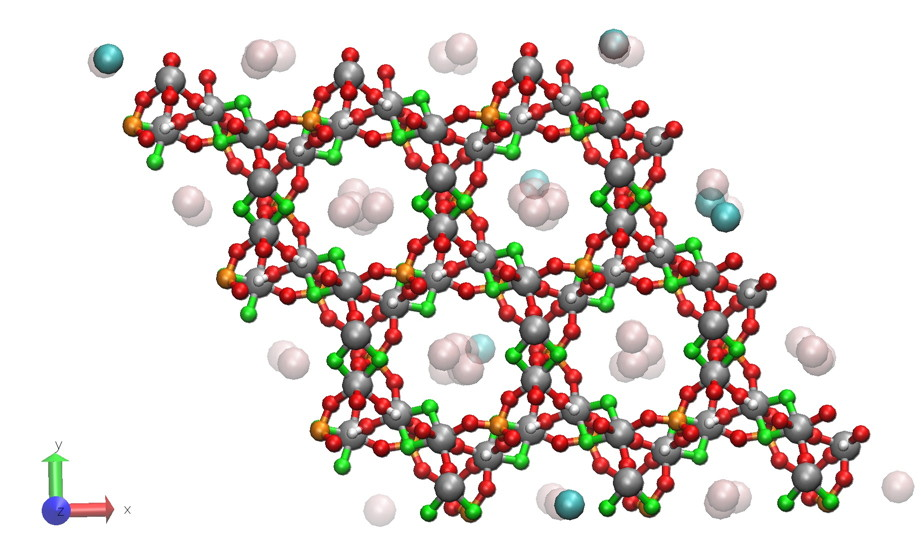
\includegraphics[width=0.48\textwidth]{figures/2-thermo/MISQIQ_clean.jpg}\hfill
    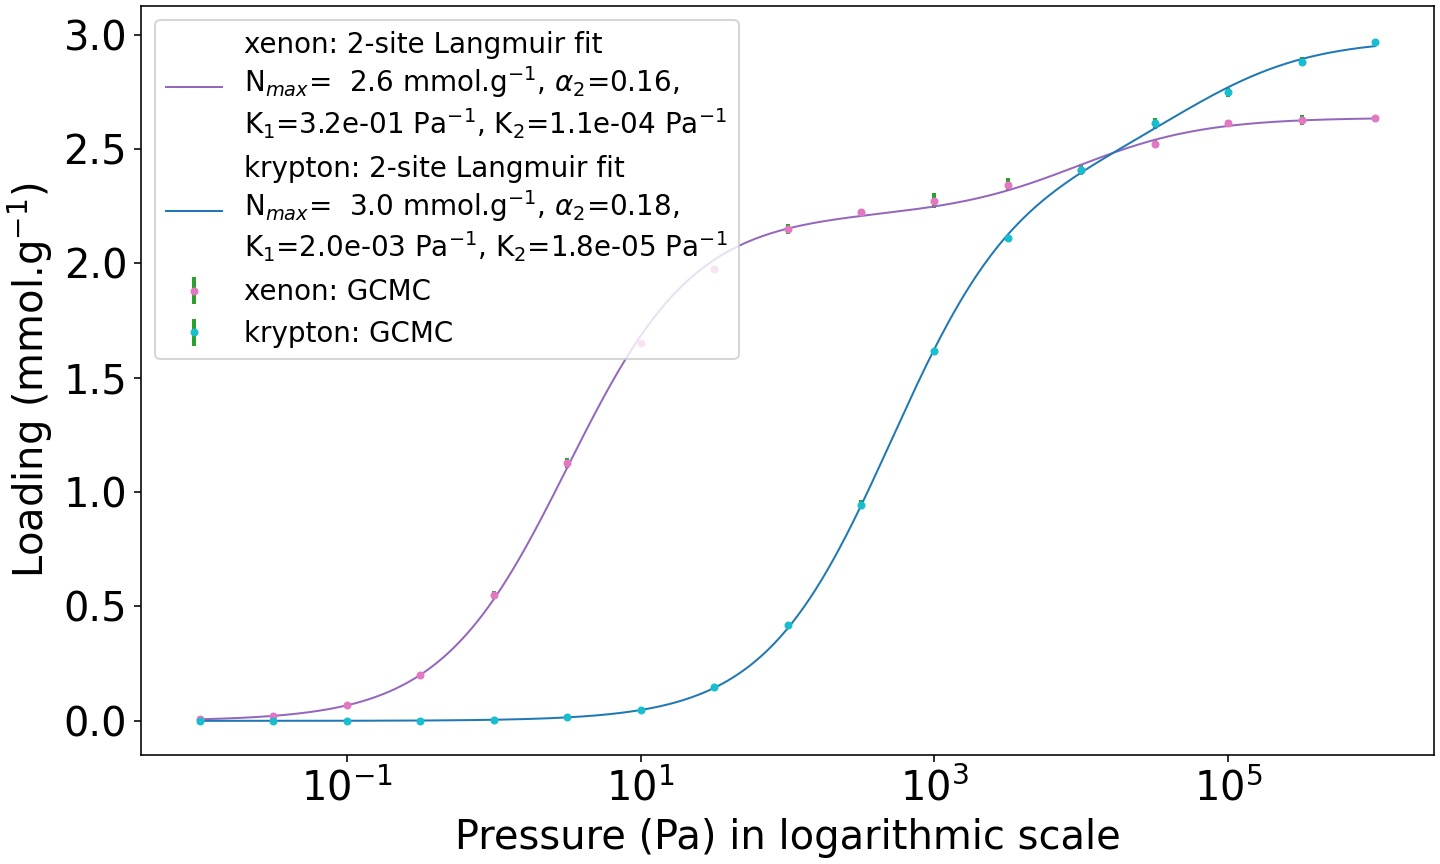
\includegraphics[width=0.48\textwidth]{figures/2-thermo/MISQIQ_clean_isotherm_xenon_krypton_298K.jpg}
    \caption{\ Representation of a chiral open-framework fluoroaluminophosphate [C$_4$N$_3$H$_{16}$]$\cdot$[Al$_6$P$_3$O$_{12}$F$_6$(OH)$_6$] denoted AlPO-JU89 (referenced MISQIQ in the Cambridge structural database), which has been loaded with xenon and krypton in a GCMC simulation, on the left side.\cite{MISQIQ} Color code: Al in silver, P in orange, O in red, H in white and F in green for the framework; and Xe in transparent pink and Kr in cyan for the adsorbates. The pure-component isotherms fitted with a 1-site Langmuir model for both xenon and krypton at \SI{298}{\kelvin} on the right side (for more information on the Langmuir parameters see supplementary information Equation~(S5)).}
    \label{fgr:MISQIQ}
  \end{figure*}
  
  We first study a few examples of the category of materials where ambient-pressure selectivity is close to (or even higher than) the low-pressure value. For VOKJIQ, the selectivity is multiplied by $1.5$ between low and ambient pressure. We see that the adsorption enthalpy of xenon $\Delta\e{ads}H\ex{Xe}$ decreases from $-53.9$\,\si{\kilo\joule\per\mol} to $-61.1$\,\si{\kilo\joule\per\mol}, whereas for krypton $\Delta\e{ads}H\ex{Kr}$ decreases from $-38.2$\,\si{\kilo\joule\per\mol} to $-44.5$\,\si{\kilo\joule\per\mol} (\emph{c.f.} supplementary information Table~S1). This increased stability of the adsorption sites upon loading is not common in nanoporous materials for rare gas adsorption, and can be linked to a cooperative effect between the adsorbed molecules. The stabilization favors the xenon molecules over the krypton molecules, due to an interatomic distance inside the pores that is a closer match to the energy well for favorable Lennard-Jones potential for xenon-xenon interactions than for krypton-krypton interactions (which is the case for a distance higher than \SI{4.2}{\angstrom}; see Figure~S10).
  
  In the case of KAXQIL, the channels are one-dimensional tubes (see Figure~S12) and the distance between two adsorption sites is approximately the unit cell parameter along the direction of the tube (\SI{5.6}{\angstrom}). There the selectivity increases with pore filling, for enthalpic reasons, which we can explain by relatively simple reasoning. The Lennard-Jones potentials $V\e{LJ}$ can be estimated for all species at \SI{5.6}{\angstrom}: $V\e{Xe-Xe}=-1.0$\,\si{\kilo\joule\per\mol}, $V\e{Kr-Kr}=-0.3$\,\si{\kilo\joule\per\mol} and $V\e{Xe-Kr}=-0.5$\,\si{\kilo\joule\per\mol}. In a simplistic model where all adsorbed molecules are \SI{5.6}{\angstrom} apart, the cooperative effect is higher between two xenon molecules, which explains the increased selectivity at high uptake. If we look further at the adsorption enthalpy of both xenon and krypton (\emph{c.f.} supplementary information Table~S1), they both increase: the guest molecules move from the ``ideal'' adsorption sites, and the guest--guest interactions do not fully compensate. The selectivity change in this material is therefore a consequence of the guest--guest interactions that rearranges the position of the adsorbates inside the nanopores.
  
  To further corroborate the role of the guest--guest interactions, we look at another material with one-dimensional tube-like channels: JUFBIX, a cobalt(II) coordination polymer based on carboxylic acid linkers (see Figure~S13).\cite{JUFBIX} The periodicity along the direction of the tubes is much higher at $7.2$\,\si{\angstrom}. The pair interaction energies corresponding to the LJ potentials at this distance are $V\e{Xe-Xe}=-0.24$\,\si{\kilo\joule\per\mol}, $V\e{Kr-Kr}=-0.06$\,\si{\kilo\joule\per\mol} and $V\e{Xe-Kr}=-0.13$\,\si{\kilo\joule\per\mol}. By looking at the adsorption enthalpies (Table \ref{tbl:effect}), these values are too small to affect the position of the adsorbed molecules. At high loading, the distance between adsorbed molecules is high, and every adsorption site is independent of the others. The ambient-pressure selectivity $s\e{1}$ is therefore the same as the low-pressure selectivity $s\e{0}$, since every guest--guest interactions are negligible. It confirms the crucial role of cooperative effects between guest molecules, when considering a saturated material.
  
  GOMREG and JAVTAC are frameworks that belong to the second category of materials, with a moderate decrease in selectivity from low to ambient pressure. In GOMREG, the channels are composed of one-dimensional tubes larger than the ones found in KAXQIL or JUFBIX (see Figure~S15 and Table~S1). The adsorption sites are alternating from left to right inside the channel, and the adsorbed molecules organize in a ``zigzag'' pattern. Looking at the adsorption enthalpies, we see that both xenon and krypton have lower enthalpies by a similar margin, suggesting an equivalent stabilization for both atoms, hence the enthalpic contribution to the selectivity change is close to 1.
  Since krypton is smaller and less strongly tied on its adsorption site than xenon, it has more available space inside the pore space. This gives an entropic advantage to the Kr, seen in the entropic contribution $k\e{S}$ of $0.64$ in Table~\ref{tbl:effect}. This indicates that even if enthalpic considerations mainly explain the observed changes at a statistical level, as discussed in the previous sections, for individual cases entropic considerations can be a strong factor in pressure-dependent selectivity.
  
  The remaining materials discussed here form a third category, with a strong decrease in selectivity from low to ambient pressure. We look at several phenomena that can be at the root of this decrease, which is important for screening studies as it can limit the working performance of a material that appears to be a ``top performer'' based on zero-pressure screening.
  
  
  For example, GOMRAC has a similar structure compared to GOMREG (see Figure~S17), except for the fact that the pores and channels are smaller (see the values of $D_f$ the diameter of the largest free sphere, and $D_i$ the diameter of the largest included sphere, in Table~S1). The distances between the adsorbed molecules --- in their ideal sites --- are then consequently smaller. At such distances, we can assume that the interactions between adsorbates become more stabilising for krypton than for xenon molecules in GOMRAC (see LJ potentials at distance lower than \SI{4.2}{\angstrom} in the Figure~S10), which translates into an enthalpic contribution $k\e{H}$ of $0.58$. Moreover, this is compatible with the equivalent guest--guest interactions in GOMREG, as previously discussed. It explains why difference between the adsorption enthalpies become smaller for GOMRAC, whereas it stays the same for GOMREG (between low and ambient pressure). This further validates the crucial role of the interactions between adsorbed molecules, and their relationship with the guest-guest distances when considering a high loading condition.
  
  If we look at the case of MISQIQ, we see that the pure-component Xe isotherm in Figure~\ref{fgr:MISQIQ} cannot be fitted by a single-site Langmuir isotherm, but is well-fitted by a two-site Langmuir model (see Figure~S18). Visual inspection of the adsorbed density at various loadings shows that this is not a second, separate adsorption site that is populated at high loading: instead, the second step in the isotherm (representing about {20\%} of the uptake at full loading) is associated with a reorganization of the adsorbate molecules occurs at high loading, accompanying a contraction of the interatomic distances. In this case, the potential for reorganization of the adsorbate in the material's nanopores leads to the change in selectivity. This reorganization can be detected on the basis of the xenon isotherm alone, and has a major role in the selectivity at ambient pressure. This repacking of the adsorbed phase is linked to a strong entropic effect, and also impacts the enthalpic contribution to selectivity.
  
  More extreme cases of selectivity drop can occur when more than one site is available, as is the case for materials BAEDTA01, VIWMOF, LUDLAZ, WOJJOV, and VAPBIZ. The pure-component isotherms and the representation of the materials loaded in xenon and krypton molecules (presented in supporting information Figures~S19-23) confirm the existence of at least two distinct adsorption sites in each material. The most selective sites (i.e., the most favorable for Xe) are filled in priority at low loading, and the less selective sites will then be populated when the pressure increases, leading to a net selectivity drop at ambient pressure for these materials. The different types of adsorption sites, and therefore the potential for a drop in Xe/Kr selectivity (at non-zero pressure) is a factor that could be explicitly included in screening of pure-component isotherms, without the need for explicit multi-component GCMC simulations.

  \subsection{Conclusions and perspectives}

  In the current state of the art on Xe/Kr separation by adsorption in nanoporous materials, many studies have focused on the determination of structure/property relationships, the description of theoretical limits of performance, and the identification of top-performing materials, whether for existing experimental structures or for novel hypothetical structures yet to be synthesized. Here, we provide a study based on a high-throughput screening of the adsorption of Xe, Kr, and Xe/Kr mixtures in 12,020 experimental open-framework materials, in order to provide a better comprehension of the thermodynamics behind Xe/Kr separation in nanoporous materials and the microscopic origins of Xe/Kr selectivity at both low and ambient pressure. 

The statistical correlation found between Henry's constant for Xe and Xe/Kr selectivity showed that the most selective materials are those with the highest affinity for xenon. To some degree of accuracy, we conclude that directly screening for Kr adsorption or for Xe free energy may not be necessary for a coarse-grained evaluation of a nanoporous framework selectivity. This could help build more efficient screening methodologies, for example with multistep studies with a first rough selection on Henry's constant at a low computational cost, followed by more expensive GCMC simulations on the selected materials (a gain that can be between 5 and 10-fold in our setup). Furthermore, inspection of the correlations between enthalpy and entropy contributions at low pressure showed that the adsorption-based separation process in the open-frameworks studied is mainly enthalpic in nature. We intend to extend the study in the future to other classes of nanoporous materials beyond MOFs, including covalent organic frameworks, porous aromatic frameworks, purely inorganic porous frameworks such as zeolites, but also amorphous porous materials such as porous polymer membranes.

In order to use nanoporous materials to separate xenon from krypton, pressure swing adsorption (PSA) processes have been widely proposed: pressure is therefore a crucial thermodynamic variable in the separation cycle. Here, we studied the difference of selectivity between a system under very low pressure (at the zero loading limit, which is calculated at relatively low computational cost) and a system at ambient pressure (closer to working conditions, but obtained at higher simulation cost). We demonstrated that the selectivity could be highly dependent on the pressure, with high low-pressure selectivity that could be maintained in some materials at ambient-pressure selectivity, while in others there would be a large drop in selectivity: a high ambient-pressure selectivity requires high low-pressure selectivity, but the reverse does not hold.

Using a thermodynamic approach to describe the separation selectivity, we showed that the differences in selectivity between the different pressures (and therefore different loading regimes of the frameworks) are mainly explained by the evolution of the adsorption enthalpies for Xe and Kr. By focusing on specific examples, we uncovered the microscopic origins of these selectivity changes, and related them to the relative roles of host--guest and guest--guest interactions. Population of different adsorption sites, or repacking of the adsorbed phase at higher loading, can lead to drastic changes in the overall selectivity. The mechanisms behind selectivity at high pressure are complex and unique to each framework, requiring a good understanding of the interactions between guest molecules constrained in the nanopores. Nevertheless, our classification of the interactions at play can help in the future to design more efficient high-throughput screening procedures.

\todo{transition to raess}

\OnlyInSubfile{\printglobalbibliography}

\end{document}
